\documentclass[10pt,twocolumn,twoside]{IEEEtran}
\usepackage{amsmath}
\usepackage{amsthm}
\usepackage{amsfonts}
\usepackage{amssymb}
\usepackage{bm}
\usepackage{microtype}
\usepackage[margin=0.8in]{geometry}
\usepackage{mathrsfs}
\usepackage{mathtools}
\usepackage{graphicx}
\usepackage{cite}
\usepackage{epstopdf}
\epstopdfsetup{outdir=./}
\DeclareMathOperator*{\argmin}{arg\,min}
\DeclareMathOperator*{\argmax}{arg\,max}
\newtheorem{definition}{Definition}
\newtheorem{lemma}{Lemma}
\newtheorem{theorem}{Theorem}
\newtheorem{problem}{Problem}
\usepackage{algorithm}
\usepackage{algpseudocode}
\newcommand{\vv}[1]{\mbox{\boldmath $#1$}}
\newcommand{\norm}[1]{\left|\left|#1\right|\right|_2}
\newcommand{\showuc}[1]{\MakeUppercase{#1}}
\newcommand{\manuallabel}[2]{\def\@currentlabel{#2}\label{#1}}
\algrenewcommand\alglinenumber[1]{\scriptsize #1}
\def \ETx {\mathcal{E}}
\def \TRx {\Gamma}	
\makeatletter
\let\OldStatex\Statex
\renewcommand{\Statex}[1][3]{%
  \setlength\@tempdima{\algorithmicindent}%
  \OldStatex\hskip\dimexpr#1\@tempdima\relax}
\makeatother
\algdef{SE}[DOWHILE]{Do}{DoWhile}{\algorithmicdo}[1]{\algorithmicwhile\ #1}
\title{}

\author{
\thanks{}
}

\begin{document}
\maketitle
\thispagestyle{empty}
\pagestyle{empty}
\begin{abstract}
\end{abstract}


\begin{IEEEkeywords}
\end{IEEEkeywords}

\section{Notations}
% !TEX root = main.tex
The transmitter energy arrival instants are marked by $t_i$'s with energy $\ETx_i$'s for $i \in \{0,1,..\}$. The transmitter has $\ETx_0$ amount of energy at time $t_0=0$. The total energy harvested at the transmitter till time $t$ is given by $\ETx(t)=\sum\limits_{i:t_i < t}\ETx(t)$. Note that $\ETx(t)$ is a staircase like function.
 
The receiver spends a constant $P_{r}$ amount of power to be in `\textit{on}' state during which it can receive data from the transmitter. When it is in `\textit{off}' state it cannot receive data, and uses no power. Hence each energy arrival (say of amount $E$) at the receiver can be viewed as adding $\TRx_i=\dfrac{E}{P_{r}}$ amount of time for which the receiver can be \textit{on}. The instances of energy arrival (which can also be thought of as `\textit{time}' arrivals) at the receiver are denoted by $r_i$. Note that transmitter can only send bits if and only if receiver is \textit{on}. The maximum amount of time for which the receiver (and hence the transmitter) can be \textit{on} assuming no energy arrives at the receiver after time '$t$' is given by the function $\TRx(t)=\sum\limits_{i:t_i\leq t} \TRx_i$.

The rate at which bits are transmitted with power `$p$' is given by function $g(p)$. The function $g(.)$ is assumed to possess the following properties. 
\begin{align}
&P1) &&g(0)=0\text{ and }\lim_{x\rightarrow \infty} g(x)= \infty,\label{property_0_infty}
\\
&P2) &&g(x)\text{ is concave in nature with } x,\label{property_concave}
\\
&P3) &&g(x)\text{ is monotonically increasing with } x,\label{property_increasing}
\\ 
&P4) &&\frac{g(x)}{x} \text{ is convex, monotonically decreasing} \nonumber
\\
&    &&\text{ with } x \text{ and } \lim_{x\rightarrow \infty} \frac{g(x)}{x}= 0.\label{property_decreasing}
\end{align}

%Any policy used for transmission is represented in form of $\{\bm{p},\bm{s},N\}$, where $N\in \mathbb{N}$, $\bm{p}=[p_1\ p_2\ ..\ p_N]$ and $\bm{s}=[s_1\ s_2\ ..\ s_{N+1}]$. The transmitter starts transmitting at time instant $s_1$ with power $p_1$ and continues till time $s_2$. From $s_2$ it transmits with power $p_2$ and so on. The policy ends at time $s_{N+1}$. 

Suppose in a transmission policy, the transmitter starts transmitting at time $s_1$ with power $p_1$ and continues till $s_2$. From $s_2$ it transmits with power $p_2$ and so on. In general, $p_i$ is the power of transmission from $s_i$ to $s_{i+1}$. The last section of transmission begins at time $s_N$ with power $p_N$, where $N\in \mathbb{N}$. The transmission ends at time $s_{N+1}$. The transmitter cannot transmit any bits when the receiver is \textit{off}. Therefore, the receiver is kept \textit{on} when transmitter transmits any bits i.e it is kept \textit{on} during the time $[s_i,s_{i+1}]$ when $p_i > 0$, $\forall \ i=1,2..,N$, and kept \textit{off} when $p_i=0$. Such a policy, sometimes referred to in this paper by the alphabets $X,Y,Z$ or $W$, is represented by the vectors $\bm{p}$, $\bm{s}$ and a number $N$, where $\bm{p}=\{p_1, p_2, .., p_N\}$ and $\bm{s}=\{s_1, s_2, .., s_{N+1}\}$. The total time for which the receiver is \textit{on} is referred to as `transmission time' or `transmission duration' and the time by which the policy get over, is called as the `finish time'. The energy used by this policy at the transmitter upto time `$t$' is given by the function $U(t)$, and the number of bits sent by time $t$ is represented by $B(t)$. Clearly,

%Such a policy is represented by the notation $\{\bm{p},\bm{s},N\}$, where $\bm{p}=\{p_1, p_2, .., p_N\}$ and $\bm{s}=\{s_1, s_2, .., s_{N+1}\}$. The energy used by this policy at the transmitter upto time '$t$' is given by the function $U(t)$ and the bits sent is represented by $B(t)$. Clearly,
\begin{align}
&U(t)=\sum_{i=1}^{j} p_i(s_{i+1}-s_i)+p_{j+1}(t-s_j) \text{ and }
\\
&B(t)=\sum_{i=1}^{j} g(p_i)(s_{i+1}-s_i)+g(p_{j+1})(t-s_j),
\\
&\text{where }j=\argmax_{i} \hspace{2mm}\{(t_i<t)\}.\nonumber
\end{align}
The function $\mathcal{P}(a,b)=\dfrac{\mathcal{E}(b^- )-U(a)}{b-a}$,  ($a>b$) denotes the maximum constant power with which transmitter can transmit from time $a$ to $b$, given that $U(a)$ amount of energy is already used upto time $a$. $a^-$ denotes the limiting value which approaches $a$ from the left.

%For convenience of presentation, we also follow the following convention : we use the notation $\stackrel{L1}{=}$ or $\stackrel{(1)}{=}$ or $\stackrel{P1}{=}$ or $\stackrel{T1}{=}$ to indicate that the equality "$=$" follows from Lemma 1 / Equation (1) / Property 1 / Theorem 1 respectively (same for inequalities).

\section{OPTIMAL OFFLINE ALGORITHM}
% !TEX root = ICC.tex
We consider an off-line scenario, which means we know all $t_i$'s and $\ETx_i$'s, non causally. We assume that the receiver harvests energy only once (say of amount $E$) at time $r_0=0$. Hence, the receiver (and so does the transmitter) can be \textit{on} for a maximum period of $\TRx_0=\frac{E}{P_r}$. We also assume that an infinite battery capacity is available both at the transmitter and the receiver to store the harvested energy. Our objective is to complete transmission (transmit $B_0$ bits) as early as possible. This is stated as an optimization problem below.

%The transmitter is supposed to transmit all $B_0$ bits in as minimum time as possible. The problem is formally stated below.
\begin{problem}
\begin{align}
&\min_{\{\textbf{p},\textbf{s},N\}}			&& T
\\
&\text{subject to} 				&& B(T)=B_0, 
\label{pb1_constraint_bits}
\\
&     										&& U(t)\le \mathcal{E}(t)  		&&& \forall \; t\;\in\;[0,T], \label{pb1_constraint_energy}
\\
&    										&& \displaystyle\sum_{\mathclap{i=1:p_i\neq 0}}^{N}(s_{i+1}-s_i)\le \TRx_0.
\label{pb1_constraint_time}
\end{align}
\end{problem}
Constraint \eqref{pb1_constraint_energy} means that we cannot use more than available energy at any point of time till we finish transmission. \eqref{pb1_constraint_time} implies that the maximum duration of transmission cannot exceed $\TRx_0$. Note that the maximum transmission duration would reduce to $(s_{N+1}-s_1)$, as we shall see in Lemma \ref{lemma_nobreaks}.  

Before describing an algorithm to solve Problem 1, we state the following Lemmas, which shall help us construct our algorithm.
% !TEX root = OptimalOfflineICC.tex

\begin{lemma}
In an optimal solution $\{\bm{p},\bm{s},N\}$ of Problem 1, if $p_i\neq 0$, $p_i\ge p_j$ for all $i,j\in \{1,2..N\}$ and $j<i$.\footnote{\label{note1}Observe that without the receiver energy harvesting constraint \eqref{pb1_constraint_time}, $p_i\neq 0,\forall i$ from \cite{Yang} and Lemma \ref{lemma_increasing_power} is identical to  Lemma 1 in \cite{Yang}. But, as we have constraint on the total receiver time, in an optimal solution the transmitter may shut \textit{off} for some time and resume transmission when enough energy is harvested to finish transmission in the given time. Hence, $p_i$ may be $0$ in-between transmissions. Lemma \ref{lemma_increasing_power} shows that even if this happens, non-zero powers still remain non-increasing.
}
\label{lemma_increasing_power}
\end{lemma}
 
\begin{proof}
The essentially follows from concavity of $g(p)$.
%We prove this by contradiction. Assume that the optimal policy (say $X$), with $\{\bm{p},\bm{s},N\}$ violates the condition stated in Lemma \ref{lemma_increasing_power}. Let $p_i\neq 0$ be the first transmission power such that $\exists k<i:\ p_i<p_k $. Let $j$ be the maximum such index less than $i$ such that $p_i<p_j$. 
%
%%
%%\begin{lemma}
%%The transmission power in every optimal solution to Problem 1 is non-decreasing with time whenever the receiver is \textit{on}.
%%\label{lemma_increasing_power}
%%\end{lemma}
%%\begin{proof}
%%We prove this by contradiction. The following two cases arise depending on whether the receiver is \textit{on} or \textit{off}.
%
%$Case\;1:$ When $j=i-1$, the proof follows similar to Lemma 1 in \cite{Yang}.
%
%$Case\;2:$ When $j<i-1$, by our assumption on choosing $j$, $p_i>p_{j+1},..,p_{i-1}$ and $p_i<p_{j}$. So, $p_{i-1},..,p_{j+1}<p_j$. Since $i$ is the  minimum index violating the condition stated in Lemma \ref{lemma_increasing_power}, $p_{i-1},..,p_{j+1}=0$. Now, consider a policy $W$ where the transmission power is same as the optimal policy before time $s_j$ and after time $s_{i+1}$. From $s_j$ to $s_j'=s_j+s_{i}-s_{j+1}$, $W$ keeps the receiver \textit{off} (so transmitter does not transmit in this duration) and from $s_j'$ to $s_{i}$ it transmits at power $p_j$. This policy still transmits equal number of bits and ends at the same time as the optimal policy $X$. Now that $W$ reduces to the structure of $X$ in \textit{Case 1} from time $s_j'$ to $s_{i+1}$ and the proof would follow similarly.



%\footnote{\label{note1}Observe that w/o receiver energy harvesting constraint \eqref{pb1_constraint_time}, $p_i\neq 0,\forall i$ from \cite{Yang} and Lemma \ref{lemma_increasing_power} would be same as Lemma 1 in \cite{Yang}. But, as we have constraint on the total receiver time, in optimal solution, transmitter may shut \textit{off} for some time and resume transmission when enough energy is harvested to finish transmission in the given time. Hence, $p_i$ may be $0$ in-between transmission. Lemma \ref{lemma_increasing_power} shows that even if this happens, non-zero powers still remain non-increasing.}  
%\label{lemma_increasing_power}
%\end{lemma}
%\begin{proof}
%We prove this by contradiction. Assume that the optimal policy (say $X$), with $\{\bm{p},\bm{s},N\}$ violates the condition stated in Lemma \ref{lemma_increasing_power}. Let $p_i\neq 0$ be the first transmission power such that $\exists k<i:\ p_i<p_k $. Let $j$ be the maximum such index less than $i$ such that $p_i<p_j$. 
%
%%
%%\begin{lemma}
%%The transmission power in every optimal solution to Problem 1 is non-decreasing with time whenever the receiver is \textit{on}.
%%\label{lemma_increasing_power}
%%\end{lemma}
%%\begin{proof}
%%We prove this by contradiction. The following two cases arise depending on whether the receiver is \textit{on} or \textit{off}.
%
%$Case\;1:$ Suppose $j=i-1$. This situation is shown in Fig. \ref{Lemma1} (a). In this case, consider a new transmission policy (say $Y$) which is same as the optimal policy till time $s_{i-1}$. From $s_{i-1}$ to $s_{i+1}$, $Y$ transmits at a constant power $p'=\dfrac{p_i(s_{i+1}-s_{i})+p_{i-1}(s_{i}-s_{i-1})}{s_{i+1}-s_{i-1}}$. Then the number of bits transmitted by policy $Y$ from time $s_{i-1}$ to $s_{i+1}$ is given by $g(p')(s_{i+1}-s_{i-1})$ while the optimal policy transmits $g(p_i)(s_{i+1}-s_{i})+g(p_{i-1})(s_{i}-s_{i-1})$ bits. Due to concavity of $g(p)$,
%\begin{align*}
%&g(p_i)\frac{s_{i+1}-s_{i}}{s_{i+1}-s_{i-1}}+g(p_{i-1})\frac{s_{i}-s_{i-1}}{s_{i+1}-s_{i-1}}
%\\ 
%&\le g\left(\frac{p_i(s_{i}-s_{i-1})+p_{i-1}(s_{i+1}-s_{i})}{s_{i+1}-s_{i-1}}\right),
%\\
%& g(p')(s_{i+1}-s_{i-1})
%\\
%&\ge g(p_i)(s_{i+1}-s_{i})+g(p_{i-1})(s_{i}-s_{i-1}).  
%\end{align*}
%Hence, both $X$ and $Y$ transmit equal number of bits till time $s_{i-1}$, while $Y$ transmits more number of bits than $X$ by time $s_{i+1}$. After time $s_{i+1}$, suppose policy $Y$ follows same transmission powers as $X$ till it transmits $B_0$ bits. Since $Y$ has transmitted more bits than $X$ till time $s_{i+1}$, it finishes transmitting all $B_0$ bits earlier than $X$, contradicting the optimality of $X$.
%
%$Case\;2:$ When $j<i-1$, by our assumption on choosing $j$, $p_i>p_{j+1},..,p_{i-1}$ and $p_i<p_{j}$. So, $p_{i-1},..,p_{j+1}<p_j$. If any of $p_{i-1},..,p_{j+1}$ is non zero, then $i$ no longer remains the minimum index violating the condition stated in Lemma \ref{lemma_increasing_power}. Hence, $p_{i-1},..,p_{j+1}=0$. This situation is shown in Fig. \ref{Lemma1}(b). Now, consider a policy $W$ where the transmission power is same as the optimal policy before time $s_j$ and after time $s_{i+1}$. From $s_j$ to $s_j'=s_j+s_{i}-s_{j+1}$, $W$ keeps the receiver \textit{off} (so transmitter does not transmit in this duration) and from $s_j'$ to $s_{i}$ it transmits at power $p_j$. This policy still transmits equal number of bits and ends at the same time as the optimal policy $X$. Now that $W$ matches with the form of $X$ in \textit{Case 1} from time $s_j'$ to $s_{i+1}$, we could proceed to generate another policy form $W$ (like $Y$ in \textit{Case 1}) which would finish earlier than $W$. Hence, this new policy would finish earlier than $X$ as well and we would reach a contradiction. 
\end{proof}

%\begin{figure}[htb]
%  \centering
%  \centerline{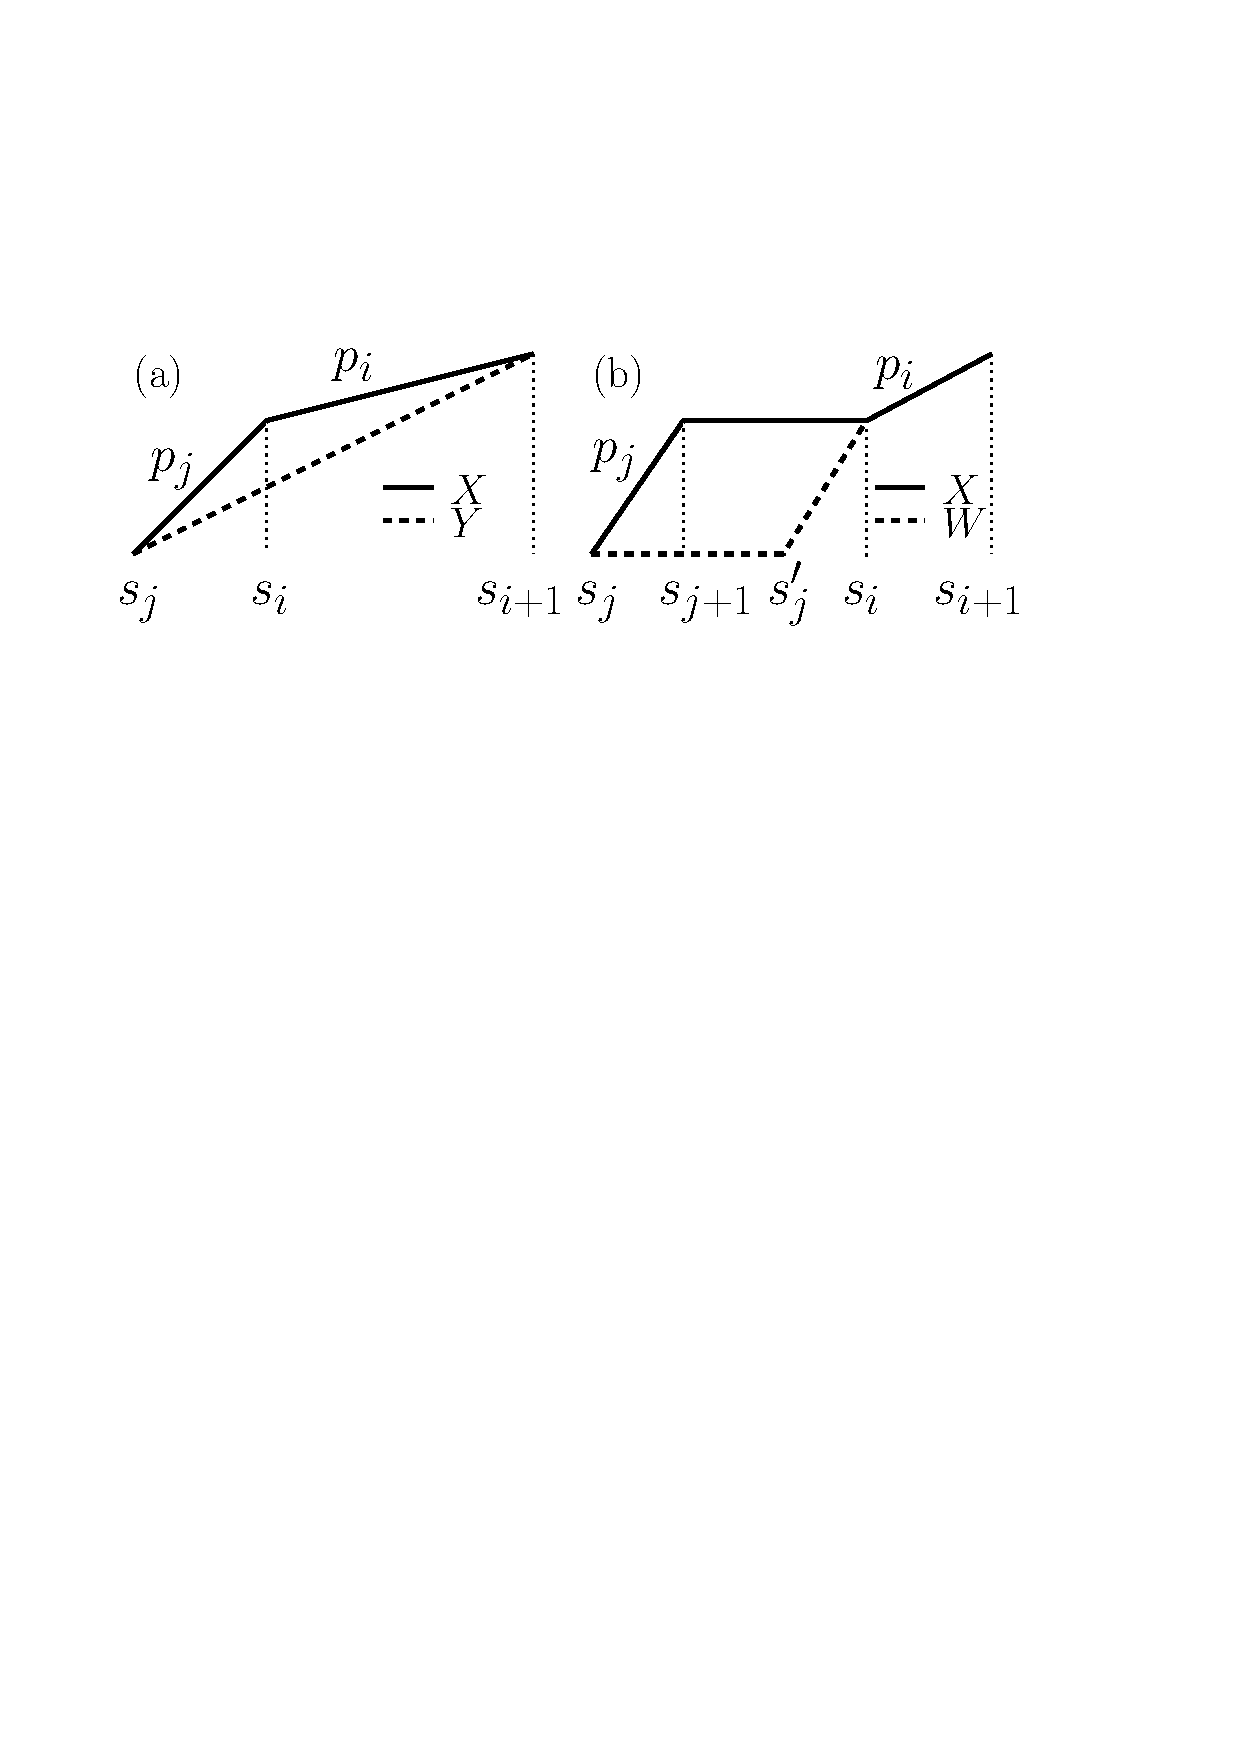
\includegraphics[width=8cm]{Lemma1.pdf}}
%\caption{Figure showing the two cases of Lemma \ref{lemma_increasing_power}, (a)\textit{Case 1}   and (b)\textit{Case 2}, with $p_i>p_j$.}\label{Lemma1}
%\end{figure}

\begin{lemma}
The optimal solution to Problem 1 may not be unique, but there always exists an optimal solution where once transmission has started, the receiver remains `\textit{on}' throughtout, until the transmission is complete. \label{lemma_nobreaks}
\end{lemma}
\begin{proof}
This is equivalent to saying that in at least one of the optimal solutions, $p_i>0$ for all $i\in\left\{ 1,2,3... N\right\}$. We prove this by showing that we can generate an optimal solution with no breaks in transmission from any other optimal solution. Let an optimal policy $X$ be characterized by $\{\bm{p},\bm{s},N\}$. Now, if $p_i\neq 0\; \forall \ i$, then we are done. Suppose some powers, say $p_{i_1},p_{i_2},...,p_{i_k}=0$ (this can happen in an optimal solution\footnotemark[\ref{note1}]) for some $k<N$, where $i_1<i_2<..<i_k$. 
%Let $p_j$ be the first non-zero power after $p_{i_1}$.

Consider a new policy (say $Y$) which is same as policy $X$ before time $s_{i_1-1}$ and after time $s_{i_1+1}$. But, it keeps the receiver \textit{off} for a duration of $(s_{i_1+1}-s_{i_1})$ starting from time $s_{i_1-1}$ (i.e. from $s_{i_1}$ to $s_{i_1}'=(s_{i_1-1}+s_{i_1+1}-s_{i_1})$) and transmits with power $p_{i_1-1}$ from time $s_{i_1}'$ till $s_{i_1+1}$. $Y$ transmits same amount of bits in same time as $X$ and also satisfies constraints \eqref{pb1_constraint_bits}-\eqref{pb1_constraint_time}. So $Y$ is also an optimal policy. But the receiver \textit{off} duration in $Y$, $(s_{{i_1+1}}-s_{i_1})$, has been shifted to left as shown in Fig.\ref{fig_Lemma2} (a). 

Next, we generate another policy $Z$ from $Y$ by shifting the \textit{off} duration $s_{i_1}'-s_{i_1-1}=(s_{{i_1+1}}-s_{i_1})$ to start from epoch $s_{i_1-2}$ upto $s_{i_1-1}'$, $s_{i_1-1}'-s_{i_1-2}=s_{i_1}'-s_{i_1-1}=(s_{{i_1+1}}-s_{i_1})$, as shown Fig. \ref{fig_Lemma2} (b). $p_{i_1-2}$  is shifted right to start from $s_{i_1-1}'$. Note that $Z$ is also optimal. We continue this process of shifting the receiver \textit{off} period to the left to generate new optimal policies till we reach a policy (say $W$) where the receiver is \textit{off} for time $(s_{{i_1+1}}-s_{i_1})$ from $s_1$, i.e. from $s_{1}$ to $s_1'$, $s_1'-s_1=(s_{{i_1+1}}-s_{i_1})$ , as shown in Fig. \ref{fig_Lemma2}(c). As $W$ has $0$ power transmission from the start $s_1$ to $s_1'$, the effective start time of $W$ can now be changed to $s_1'$. 

Similarly, we shift the receiver \textit{off} period corresponding to $p_{i_2},...,p_{i_k}$ till the total \textit{off} period is shifted to the beginning of transmission. This will result in a policy which starts \textit{after} time $s_1$ (at $s_1+(s_{{i_1+1}}-s_{i_1})+..+(s_{{i_k+1}}-s_{i_k})$) and ends at time $s_{N+1}$, but the transmission power never goes zero in-between. Such a policy is also optimal and has no breaks.
\end{proof}
\begin{figure}[htb]
  \centering
  \centerline{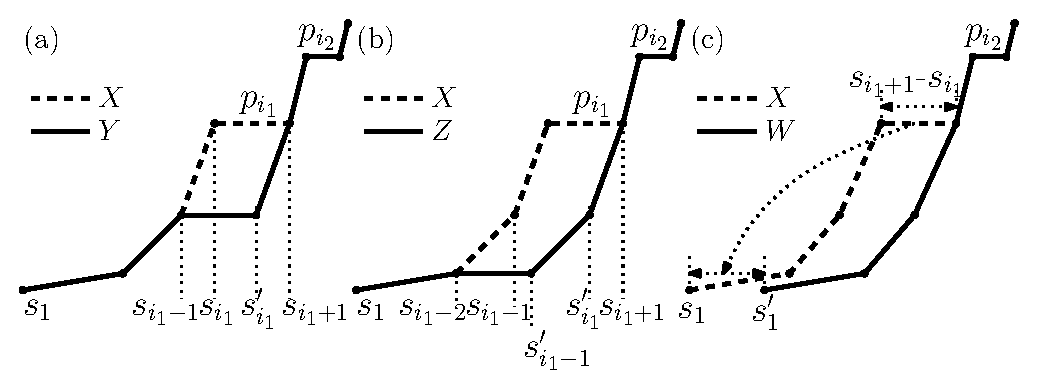
\includegraphics[width=8cm]{Lemma2.eps}}
\caption{Illustration of Lemma \ref{lemma_nobreaks}. Receiver \textit{off} time of $(s_{j}-s_{i_1})$ is progressively shifted to left as shown in (a) to (b) to (c).}\label{fig_Lemma2}
\end{figure}
\textit{In the subsequent discussion, whenever we refer to the optimal solution for Problem 1, we assume it is the one with no breaks in transmission.}
%This is equivalent to saying that there are no breaks during transmission in an optimal solution. Again, we shall prove this by contradiction. In the optimal solution, suppose the receiver is \textit{off} for some period after transmission starts. Let the transmission power before the break is $p_1$ and after the break is $p_2$. Considering Lemma \ref{lemma_increasing_power}, $p_1<p_2$, as shown in Fig. \ref{Lemma2_figure} (a). Consider the policy where we keep the receiver \textit{off} from time $A$ to $B'=(A+C-B)$. Now, an energy arrival can occur at the transmitter at any time between $A$ to $D$. If there is no energy arrival then transmitting at a constant rate from $B'$ to $D$ would transmit more bits.
%
%$Case 1:$ If the energy arrival is between $A$ and $B'$, then it can be easily seen that transmitting at a constant rate from $B'$ to $D$ would be better due to concavity of $g(p)$.
%
%$Case 2:$ If the arrival is between $B'$ and $C$ (say $C'$), then again transmitting at a same rate $p_1$ from $B'$ to $C'$ and  at a constant rate from $C'$ to $D$ would deliver more number of bits. In the worst case, an energy arrival occurring at $C$ would make this scenario transmit equal number of bits as the original scenario.
%
%$Case 3:$ If there is an energy arrival from $C$ to $D$ (say $D'$), then transmitting at maximum possible constant power form $B'$ to $D'$ and then at same rate $p_2$ from $D'$ to $D$ would deliver more bits to the receiver.
%
%Applying the above scenarios iteratively we could shift the receiver \textit{off} duration $(C-B)$ to the beginning of transmission and still, at worst case, transmit equal number of bits in same total time. Hence having a break in between transmission is always discouraged. This also gives us an idea of why the optimal solution may not be unique.
%\end{proof}
%
%\begin{figure}[htb]
%\centering
%\centerline{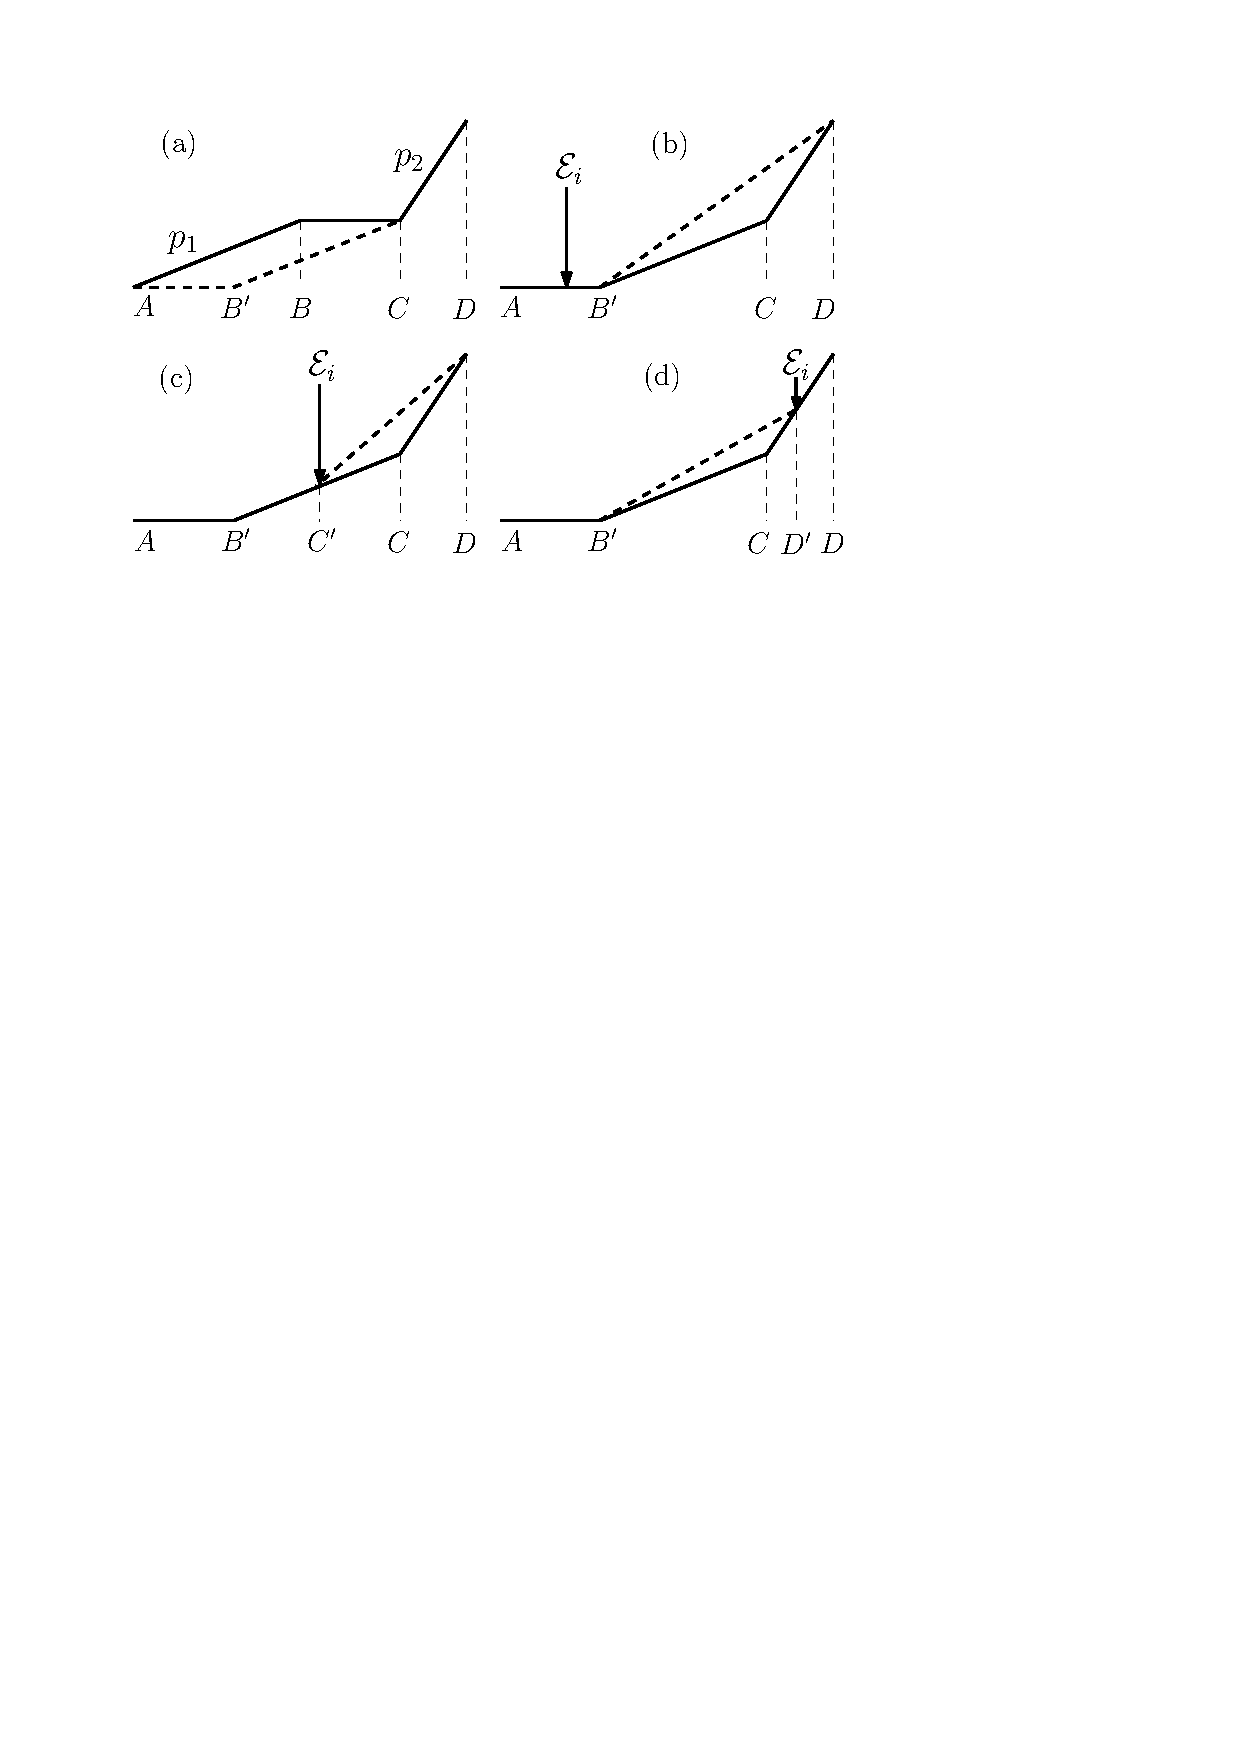
\includegraphics[width=8cm]{Lemma2.pdf}}
%\caption{Figure showing the three cases of Lemma \ref{lemma_nobreaks}, (a) the original scenario, (b) \textit{Case 1}, (c) \textit{Case 2} and (d) \textit{Case3} with $p_1>p_2$.}
%\label{Lemma2_figure}
%\end{figure}

\begin{lemma}
In an optimal policy $\{\bm{p},\bm{s},N\}$, $s_i=t_j$ for some $j$ and $U(s_i)=\ETx(s_i^-)$  ,  $\forall \;i\in\{\bm{2},3,...,N\}$. Further, $U(s_{N+1})=\ETx(s^-_{N+1})$.
\label{lemma_energy_consumed} 
\end{lemma}
\begin{proof}
Keeping in mind Lemma \ref{lemma_increasing_power} and \ref{lemma_nobreaks},  $p_i\neq 0$ and $p_{i+1}\ge p_i,\forall i\in [N]$. Assuming such a structure, the proof can be argued in similar terms of Lemma 2,3 in \cite{Yang}. 
\end{proof}	
For notational simplicity, $\bm{s}$ is assumed to exhaust all $t_k$'s, where $U(t_k)= \ETx(t_k^-)$.
  
\begin{lemma}
Consider two policies $\{\bm{p},\bm{s},N\}$  and $\{\bm{\widetilde{p}},\bm{\widetilde{s}},N\}$, which are feasible with respect to energy constraint \eqref{pb1_constraint_energy}, have non-decreasing powers and transmit same number of bits in total. If $Y$ is same as $X$ from time $s_2$ to $s_{N}$, but $\widetilde{p}_1=p_1-\alpha,\widetilde{p}_N=p_N+\beta, \widetilde{s}_1=s_1-\gamma, \widetilde{s}_N=s_N+\delta $ and $U(s_{N+1})=U(\widetilde{s}_{N+1})$, where $\alpha ,\beta,\gamma,\delta>0$, then
\begin{equation*}
(\widetilde{s}_{N+1}-\widetilde{s}_1)>(s_{N+1}-s_1).
\end{equation*}

% \textbf{one way:}
% Consider a feasible policy $X$, $\{\bm{p},\bm{s},N\}$ with non-decreasing powers. If it is possible to create another policy $Y$,$\{\bm{\widetilde{p}},\bm{\widetilde{s}},N\}$, from $X$ by keeping the transmission same as $X$ from time $s_2$ to $s_{N}$, but by decreasing $p_1$ and increasing $p_N$ such that $Y$ is also feasible with respect to energy constraint \eqref{pb1_constraint_bits}, transmits same number of bits as $X$ and uses same amount of energy by the time it finishes, then transmission time for $Y$ is more than that of $X$.
% 
% \textbf{other way:}
%Consider two policies $X$, $\{\bm{p},\bm{s},N\}$  and $Y$, $\{\bm{\widetilde{p}},\bm{\widetilde{s}},N\}$, which are feasible with respect to energy constraint \eqref{pb1_constraint_energy}, have non-decreasing powers, transmit same number of bits in total and use same amount of energy by the time they finish. If $Y$ is same as $X$ from time $s_2$ to $s_{N}$, but $\widetilde{p}_1$ is less than $p_1$ and $\widetilde{p}_N$ is more than $p_N$, then transmission time for $Y$ is more than that of $X$.

\label{lemma_increase_time}
\end{lemma}
\begin{proof} The proof involves long algebraic calculations that essentially rely on the concavity of $g(p)$ and convexity of $g(p)/p$.
%Restating our objective mathematically, if $\widetilde{p}_1=p_1-\alpha,\widetilde{p}_2=p_2,..,\widetilde{p}_{N-1}=p_{N-1},\widetilde{p}_N=p_N+\beta $ and $\widetilde{s}_1=s_1-\gamma,\widetilde{s}_2=s_2,..,\widetilde{s}_{N-1}=s_{N-1},\widetilde{s}_N=s_N+\delta $, where $\alpha ,\beta,\gamma,\delta$ are positive constants, then we need to show that $(\widetilde{s}_{N+1}-\widetilde{s}_1)>(s_{N+1}-s_1)$. The two policies $X$  and $Y$ are shown in Fig. \ref{lemma4}.
%\\
%$X$ and $Y$ having used same amount of energy, we can say that $\ETx(\widetilde{s}_2)-\ETx(\widetilde{s}_1)=\ETx(s_2)-\ETx(s_1)$ and $\ETx(\widetilde{s}_{N+1})-\ETx(\widetilde{s}_N)=\ETx(s_{N+1})-\ETx(s_N)$. Thus, we can calculate $\gamma=\dfrac{\alpha}{p_1-\alpha}(s_2-s_1)$ and $\delta =\dfrac{\beta}{p_N+\beta}(s_{N+1}-s_N)$. As $X$ and $Y$ transmit equal number of bits between time $s_2$ and $s_N$, we can just equate the number of bits transmitted by $X$ before $s_1$ and after $s_{N}$ (LHS of \eqref{Lemma4_eq1}) with that of $Y$ (RHS of \eqref{Lemma4_eq1}). Note that only one of the four variable $\alpha,\beta,\gamma,\delta$ can be independently chosen.
%\\
%\begin{align}
%&g(p_N)(s_{N+1}-s_N)+g(p_1)(s_2-s_1)\nonumber
%\\
%&=g(\widetilde{p}_N)(\widetilde{s}_{N+1}-\widetilde{s}_N)+g(\widetilde{p}_1)(\widetilde{s}_2-\widetilde{s}_1)\label{Lemma4_eq1},
%\end{align}
%Therefore,
%\begin{align}
%& (p_N+\beta)p_N\frac{\delta}{\beta}\left(\frac{g(p_N)}{p_N}-\frac{g(p_N+\beta)}{p_N+\beta}\right)\nonumber
%\\
%&=(p_1-\alpha)p_1\frac{\gamma}{\alpha}\left(\frac{g(p_1-\alpha)}{p_1-\alpha}-\frac{g(p_1)}{p_1}\right).\label{bits_equal}
%\end{align}
%As $g(p)/p$ is a continuous \& differentiable function, the mean value theorem implies that $\exists$ $p_N':p_N<p_N'<p_{N}+\beta$ and $p_1':p_1-\alpha<p_1'<p_{1}$ such that
%\begin{align}
%&\frac{d}{dp} \frac{g(p)}{p} \bigg{\vert}_{p=p_N'}=\frac{1}{\beta}\left(\frac{g(p_N+\beta)}{p_N+\beta}-\frac{g(p_N)}{p_N}\right)\text{ and }\label{diff_1}
%\\
%&\frac{d}{dp} \frac{g(p)}{p}\bigg{\vert}_{p=p_1'}=-\frac{1}{\alpha}\left(\frac{g(p_1-\alpha)}{p_1-\alpha}-\frac{g(p_1)}{p_1}\right)\label{diff_2}.
%\end{align}
%Substituting (\ref{diff_1}) and (\ref{diff_2}) in (\ref{bits_equal}) we get,
%\begin{align}
%&\delta(p_N+\beta)p_N\frac{d}{dp} \frac{g(p)}{p}  \bigg{\vert}_{p=p_N'}
%=\gamma(p_1-\alpha)p_1\frac{d}{dp} \frac{g(p)}{p} \bigg{\vert}_{p=p_1'}.\label{bits_equal1}
%\end{align}
%Since $\dfrac{d}{dp} \dfrac{g(p)}{p}$ is an increasing function of $p$ (from \eqref{property_decreasing}), with $p_1'<p_1\le p_N<p_N'$, (\ref{bits_equal1}) implies $\gamma >\delta$. Hence, transmission time in the policy $Y$, $\left( s_{N+1}-s_1+\gamma-\delta\right)$, is greater than the transmission time in policy $X$ i.e. $(s_{N+1}-s_1)$.
\end{proof}
%\begin{figure}
%\centering
%  \centerline{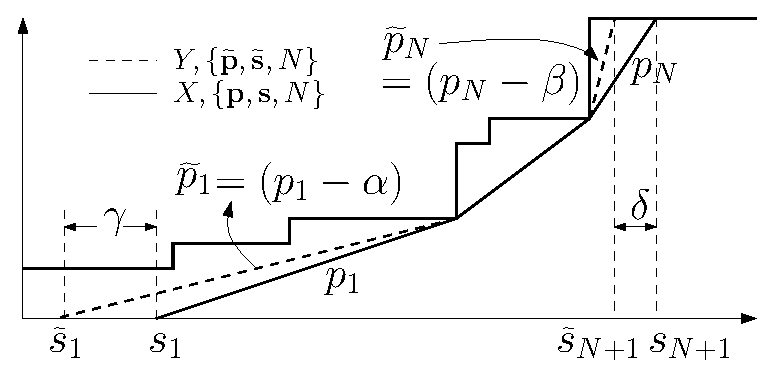
\includegraphics[width=8cm]{Lemma4.eps}}
%\caption{Illustration for the proof of Lemma \ref{lemma_increase_time}.}\label{lemma4}
%\end{figure}

\begin{lemma}
If the receiver has energy to stay \textit{`on'} for a maximum of $\TRx_0$ time, then in an optimal policy, either $s_{N+1} - s_1 = \TRx_0$ or $s_1 = 0$. 
\label{transmission_duration}
\end{lemma}
\begin{proof}
We shall prove this by contradiction. Suppose the optimal transmission policy say $X$, $\{\bm{p},\bm{s},N\}$ begins at $s_1\neq 0$ and transmits for a duration $(s_{N+1}-s_1)< \TRx_0$. We want to show that it is always possible to generate a policy which finishes earlier than $X$, having transmission time squeezed in between $(s_{N+1}-s_1)$ and $\TRx_0$. Consider another policy $Y$, $\{\bm{\widetilde{p}},\bm{\widetilde{s}},N\}$ as defined in Lemma \ref{lemma_increase_time}. As $\alpha$, $\beta$, $\delta$, $\gamma$ are all related (by constraints presented in Lemma \ref{lemma_energy_consumed}), choice of one variable (without loss of generality, say $\alpha$) independently, defines $Y$. By definition of $s_i$'s, $s_{2}$ is the first energy arrival which is on the boundary of energy constraint (\ref{pb1_constraint_energy}) i.e. $U(s_2)=\ETx(s_2^-)$ and $s_{N}$ is the last epoch satisfying $U(s_N)=\ETx(s_N^-)$. Hence, we can choose $\alpha>0$, such that $\tilde{p}_1$ and $\tilde{p}_N$ would be feasible with respect to energy constraint (\ref{pb1_constraint_energy}). Note that if $s_1=0$, then any value of $\alpha$ would have made $\widetilde{p}_1$ infeasible. From Lemma \ref{lemma_increase_time}, we know that the policy $Y$ transmits for more time than $X$. i.e. $(\tilde{s}_{N+1}-\tilde{s}_1) > (s_{N+1} - s_{1})$. Let $s_{N+1}-s_1=\TRx_0-\epsilon$, with $\epsilon >0$. If the chosen value of $\alpha$ is such that $\gamma -\delta\le\epsilon$, then $\left( \widetilde{s}_{N+1}-\widetilde{s}_1\right)<\TRx_0$. If not, then we can further reduce $\alpha$ so that $\gamma -\delta\le\epsilon$ ($\alpha$,$\beta$,$\gamma$,$\delta$ being related by continuous functions).  Note that when $\epsilon=0$ any choice of $\alpha$ would make $\left( \widetilde{s}_{N+1}-\widetilde{s}_1\right)>\TRx_0$. Hence, with this choice of $\alpha$, $(s_{N+1}-s_1)<\left( \widetilde{s}_{N+1}-\widetilde{s}_1\right)<\TRx_0$ holds and  policy $Y$ is feasible with constraints  (\ref{pb1_constraint_bits}), (\ref{pb1_constraint_energy}), (\ref{pb1_constraint_time}) and contradicts the optimality of policy $X$ (as finish time of $Y$, $\widetilde{s}_{N+1}=s_{N+1}-\delta <s_{N+1}$). This concludes that $s_{N+1}-s_1=\TRx_0$ (if $s_1\neq 0$) in optimal policy.
\end{proof}
%%!TEX root = OptimalOfflineICC.tex
%input{Siddhartha}


%\begin{algorithm}
%\caption{Off-line Algorithm for finding optimal transmission policy to Problem 1}
%\footnotesize%\scriptsize
%\label{Algorithm1}
%\begin{algorithmic}[1]
%\State \textbf{Initialization}: $\{\textbf{p},\textbf{s},N\}\gets$ INIT\_POLICY
%\State $t_l=s_2$, $t_{r}=s_{N}$, $T_{start}=s_1$, $T_{stop}=s_{N+1}$, $p_l=p_1$, $p_r=p_{N}$, $control=0$.
%\State Delete $s_1$, Delete $s_{N+1}$, Delete $p_N$, Delete $p_1$.
%%\Procedure{InitPolicy}{}
%\While {$\left(T_{stop}-T_{start}< \TRx_0\right) \text{ and } \left(T_{start}>0\right)$}
%\label{algo_while_loop}
%	\If {$\{i:t_r<t_i < T_{stop}\}=\emptyset$}
%		\State $B_l=g(p_r)(T_{stop}-t_r)+g(p_l)(t_l-T_{start})$, $control=1$.
%	\Else
%		\State $j=\displaystyle \argmin_{i:t_r<t_i < T_{stop}} \mathcal{P}(t_r,t_i)$
%		\State $B_l=g(p_r)(T_{stop}-t_r)+g(p_l)(t_l-T_{start})-g\left(\mathcal{P}(t_r,t_j)\right)						\left(\frac{\ETx(T_{stop}^-)-\ETx(t_r^-)}{\mathcal{P}(t_r,t_j)}\right) $\label{algo_bits_left_1}
%	\EndIf
%
%	\State Solve for $\tilde{p}$: $\frac{\ETx(t_l^-)}{\tilde{p}}g(\tilde{p})=B_l$\label{algo_bits_left_2}
%	\State $A=\{i:\tilde{p}t_i+(\ETx(t_l^-)-\tilde{p}t_l))> \ETx(t_i^-), \forall \left(t_l-					\frac{\ETx(t_l^-)}{\tilde{p}}\right)<t_i<t_l\}$
%
%	\If {$A=\emptyset$}
%		\State $p_l=\tilde{p}$, $T_{start}=t_l-\ETx(t_l^-)/p_l$
%		\If {$control=0$}
%			\State $p_r=\mathcal{P}(t_r,t_j)$, $T_{stop}=t_r+\frac{\ETx(T_{stop^-})-\ETx(t_r^-)}							{\mathcal{P}					(t_r,t_j)}$
%			\State $t_r=t_j$, $\textbf{p}.append(\mathcal{P}(t_r,t_j))$, $\textbf{s}.append( t_j)$ 
%		\Else
%			\State $T_{stop}=t_r$, $t_r=\textbf{s}.last$, $p_r=\textbf{p}.last$
%			\State Delete $\textbf{s}.last$, Delete $\textbf{p}.last$
%			\State $control=0$
%		\EndIf
%	\Else 
%		\State $k=\displaystyle \argmax_{i:\max\left(\left(t_l-\ETx(t_l^-)/\tilde{p}\right),0\right)					\le t_i <t_l} \mathcal{P}(t_i,t_l)$
%		\State $B_r=g(p_r)(T_{stop}-t_r)+g(p_l)(t_l-T_{start})-g\left(\mathcal{P}(t_k,t_l)\right)							\left(\frac{\ETx(T_{start}^-)}{\mathcal{P}(t_k,t_l)}\right)$
%		\State $p_l=\mathcal{P}(t_k,t_l)$, $T_{start}=t_l-\ETx(t_l^-)/\mathcal{P}(t_k,t_l)$
%		 
%		\State $t_l=t_k$, $\textbf{p}.prepend=p_l$, $\textbf{s}.prepend=t_k$
%	
%		\State Solve for $p_r$: $\frac{\ETx(T_{stop}^-)-\ETx(t_r)}{p_r}g(p_r)=B_r$
%		\State $T_{stop}=t_r+(\ETx(T_{stop}^-)-\ETx(t_r^-))/p_r$	
%	\EndIf
%
%\EndWhile
%
%\If {$(T_{start}-T_{stop})>\TRx_0$}
%	\State $T=\TRx_0-(t_r-t_l)$, $B=B_0-\displaystyle\sum_{i}g(p_i)(s_{i+1}-s_{i})$
%	\State Solve for  $x$: $xg\left(\dfrac{\ETx(t_{l}^-)}{x}\right)+\left(T-x\right) g 		\left(\dfrac{\ETx(t_{stop}^-)-\ETx(t_{r}^-)}{T-x}\right) = B$(with prev iteration $t_l$ and $t_r$)\label{algo_solve_eqn}
%	\State $p_l=\dfrac{\ETx(t_{l}^-)}{x}$, $T_{start}=t_l-x$
%	\State $p_r=\dfrac{\ETx(t_{stop}^-)-\ETx(t_{r}^-)}{T-x}$, $T_{stop}=t_r+T-x$
%\EndIf
%
%\State $\textbf{p}.prepend(p_l)$, $\textbf{s}.prepend(T_{start})$, $\textbf{p}.append(p_r)$, $\textbf{s}.append(T_{stop})$
%\State \Return $\{\textbf{p},\textbf{s}, \text{number of elements in \textbf{p}}\}$ 	 
%%\EndProcedure
%\end{algorithmic}
%\end{algorithm}


\begin{theorem}
A transmission policy $\{\textbf{p},\textbf{s},N\}$ is an optimal solution to Problem 1 if and only if it satisfies the following structure.
\label{th_algo1_1}
\begin{align}
&\sum_{i=1}^{i=N}g(p_i)(s_{i+1}-s_i)=B_0; 								
\label{claim1}
\\
&p_1\le p_2 ..\le p_N;
\label{claim3}  
\\
&\nonumber s_i=t_j \text{ for some } j, i\in \{2,..,N\} \ \text{ and }
\\
& U(s_i)=\ETx(s_i^-), \forall i\in \{2,..,N+1\};
\label{claim4}
\\
&\nonumber s_{N+1}-s_1=\mathcal{R}_0, 	 \ \ \ \ 						\text{ if } s_1>0 \text{ or }
\\
& s_{N+1}\le \mathcal{R}_0,				\ \ \ \ \ \ \ \ \ \				\text{ if } s_1=0;
\label{claim2}
\\
&\exists s_j:s_j\in \textbf{s} \text{ and } s_j=t_q.
\label{claim5}
\end{align}
%& \nonumber s_{n+1}=\argmin_{t_i: s_n < t_i \le s_{N+1}} \mathcal{P}(s_n,t_i)=\dfrac{\ETx(t_i^-)-U(s_n)}{t_i-s_n} \	\text{ and }
%\\
%&p_n=\mathcal{P}(s_{n},s_{n+1});\label{claim3}							
%\\
\end{theorem}
\begin{proof}

%The proof consists of establishing both necessary and sufficiency conditions. First we work out the necessary part i.e. an optimal policy, say $X$, $\{\textbf{p},\textbf{s},N\}$ must have the given structure. We prove it by contradiction. We establish structure (\ref{claim3}) at first. Assume the optimal policy $X$ satisfies Lemmas \ref{lemma_increasing_power}-\ref{lemma_Q} and does not satisfy structure (\ref{claim3}). Specifically, say the policy abides by the  structure (\ref{claim3}) from time $s_{1}$ to $s_n$, for some $n\in \{1,2,..,N\}$ but transmission power right after $s_n$ is not the minimum feasible constant power, i.e.
%\begin{align}
%p_n>\mathcal{P}(s_n,\tilde{s})\text{ where } \tilde{s}=\argmin_{t_i: s_n < t_i \le s_{N+1}} \mathcal{P}(t_i,s_n).\label{claim3_1}
%\end{align}
%Note that $p_n$ is not less than $\mathcal{P}(s_n,\tilde{s})$, as $\mathcal{P}(s_n,\tilde{s})$ is the minimum feasible power among all the epochs. The maximum energy that can used for transmission from time $s_{n}$ to $\tilde{s}$ is $\left(\ETx(\tilde{s}^-)-\ETx(s_{n}^-)\right)$, since the optimal policy has used all the energy till time $s_{n}^-$, by Lemma \ref{lemma_energy_consumed}. If $\tilde{s}<s_{n+1}$, the transmission policy uses $p_n(\tilde{s}-s_{n})$ energy from time $s_n$ to $\tilde{s}$. If $\tilde{s}>s_{n+1}$, the transmission power during time $[s_{n+1},\tilde{s}]$ has to be greater than or equal to $p_n$ by Lemma \ref{lemma_increasing_power}. So the total energy used during period $[s_n,\tilde{s}]$ can be lower bounded by $p_n(\tilde{s}-s_{n})$. But, this energy is always more than the maximum energy available from $s_{n}$ to $\tilde{s}$ because
%\begin{align}
%&\nonumber\ETx(\tilde{s}^-)-\ETx(s_{n}^-)=\mathcal{P}(s_n,\tilde{s})(\tilde{s}-s_{n})<p_n(\tilde{s}-s_{n}),
%\end{align}
%where the inequality follows from (\ref{claim3_1}). This violates constraint (\ref{pb1_constraint_energy}) and contradicts the optimality of $X$.
%
%Moving on to other structures, (\ref{claim1}) must be followed by the optimal policy as it is a constraint to the Problem 1, (\ref{claim4}) follows from Lemma \ref{lemma_Q} and \eqref{claim2} follows from Lemma \ref{transmission_duration}.


The proof consists of establishing both necessary and sufficiency conditions. First we work out the necessary part i.e. an optimal policy must have the given structure. Observing the structure, (\ref{claim1}) must be followed by the optimal policy as it is a constraint to the Problem 1, \eqref{claim3} follows from Lemma \ref{lemma_increasing_power}, \ref{lemma_nobreaks}, \eqref{claim4} follows from Lemma \ref{lemma_energy_consumed}, \eqref{claim2} follows from Lemma \ref{transmission_duration} and \eqref{claim5} follows from Lemma \ref{lemma_Q}.



%We are left to prove structure (\ref{claim2}). $s_{N+1}-s_1\le \mathcal{R}_0$ by constraint (\ref{pb1_constraint_time}). If $s_1=0$ then we are done. When $s_1>0$, assume that $s_{N+1}-s_1<\mathcal{R}_0$. Now consider the policy where power vector is given by $\bm{\widetilde{p}}=\{p_1-\alpha,p_2,..,p_{N-1},p_N+\beta \}$ and the corresponding time vector be given by $\bm{\widetilde{s}}=\{s_1-\gamma,s_2,..,s_{N},s_{N+1}-\delta\}$, where $\gamma=\dfrac{\alpha}{p_1-\alpha}(s_2-s_1)$, $\delta =\dfrac{\beta}{p_N+\beta}(s_{N+1}-s_N)$ and $\alpha ,\beta$ are small positive constants. Since $(s_{N+1}-\delta)>s_{N+1}$, this policy finishes before the optimal policy $\{\textbf{p},\textbf{s},N\}$ and hence amounts to a contradiction only if we are able to show that it is feasible. By the definition of $s_i$ in (\ref{claim3}), $s_{2}$ is the first energy arrival which is on the boundary of energy constraint (\ref{pb1_constraint_energy}) i.e. $U(s_2)=\ETx(s_2^-)$ and $s_{N}$ is the last epoch satisfying $U(s_N)=\ETx(s_N^-)$. So we can choose arbitrarily small $\alpha ,\beta$ such that policy $\{\bm{\widetilde{p}},\bm{\widetilde{s}},N\}$ would be feasible with respect energy constraint (\ref{pb1_constraint_energy}). For every $\beta\rightarrow 0^+$ we can find a value of $\alpha$ such that the number of bits transmitted in policy $\{\bm{\widetilde{p}},\bm{\widetilde{s}},N\}$ remains the same as policy $\{\textbf{p},\textbf{s},N\}$ i.e. equal to $B_0$. So, excluding the common parts in the transmission policy $\{\textbf{p},\textbf{s},N\}$ and $\{\bm{\widetilde{p}},\bm{\widetilde{s}},N\}$, we can equate
%\begin{align}
%&g(p_N)(s_{N+1}-s_N)+g(p_1)(s_2-s_1)\nonumber
%\\
%&=g(p_1-\alpha)(s_2-s_1+\gamma)+g(p_N+\beta)(s_{N+1}-s_N-\delta)\nonumber,
%\\
%&\implies \delta(p_N+\beta)p_N\frac{1}{\beta}\left(\frac{g(p_N)}{p_N}-\frac{g(p_N+\beta)}{p_N+\beta}\right)\nonumber
%\\
%&=\gamma(p_1-\alpha)p_1\frac{1}{\alpha}\left(\frac{g(p_1-\alpha)}{p_1-\alpha}-\frac{g(p_1)}{p_1}\right).\label{bits_equal}
%\end{align}
%$\exists$ $p_N':p_N<p_N'<p_{N}+\beta$ and $p_1':p_1-\alpha<p_1'<p_{1}$ such that
%\begin{align}
%&\frac{d}{dp} \frac{g(p)}{p} \bigg{\vert}_{p=p_N'}=\frac{1}{\beta}\left(\frac{g(p_N+\beta)}{p_N+\beta}-\frac{g(p_N)}{p_N}\right),\label{diff_1}
%\\
%&\frac{d}{dp} \frac{g(p)}{p}\bigg{\vert}_{p=p_1'}=-\frac{1}{\alpha}\left(\frac{g(p_1-\alpha)}{p_1-\alpha}-\frac{g(p_1)}{p_1}\right)\label{diff_2}.
%\end{align}
%Substituting (\ref{diff_1}) and (\ref{diff_2}) into (\ref{bits_equal}) we get,
%\begin{align}
%&\delta(p_N+\beta)p_N\frac{d}{dp} \frac{g(p)}{p}  \bigg{\vert}_{p=p_N'}
%=\gamma(p_1-\alpha)p_1\frac{d}{dp} \frac{g(p)}{p} \bigg{\vert}_{p=p_1'}.\label{bits_equal1}
%\end{align}
%It can be verified that $\dfrac{d}{dp} \dfrac{g(p)}{p}$ is decreasing function of $p$. As $p_1'<p_N'$, equation (\ref{bits_equal1}) implies $\gamma >\delta$. Hence the time for which transmission occurs in the policy $\{\bm{\widetilde{p}},\bm{\widetilde{s}},N\}$, $\left( s_{N+1}-s_1+\gamma-\delta\right)$, is greater than transmission time in policy $\{\textbf{p},\textbf{s},N\}$ i.e. $(s_{N+1}-s_1)$. As $s_{N+1}-s_1<\TRx_0$, we can choose arbitrarily small positive value of $\beta$ so that $(s_{N+1}-s_1)<(s_{N+1}-s_1+\gamma -\delta)<\TRx_0$ holds. So policy $\{\bm{\widetilde{p}},\bm{\widetilde{s}},N\}$ is feasible with constraints  (\ref{pb1_constraint_bits}), (\ref{pb1_constraint_energy}), (\ref{pb1_constraint_time}) and contradicts the optimality of policy $\{\textbf{p},\textbf{s},N\}$. This concludes that $s_{N+1}-s_1=\TRx_0$ (if $s_1\neq 0$) in optimal policy.

Next, we prove the sufficiency of the structure. Let a policy $X$, $\{\textbf{p},\textbf{s},N\}$ follow  structure \eqref{claim1}-\eqref{claim5}. We need to show that this policy is optimal. We adopt the method of contradiction to prove this. Assume that it is not true. So, there exists another policy $Y$, $\{\textbf{p'},\textbf{s'},N'\}$ which is optimal. $Y$ abides by the Lemma \ref{lemma_increasing_power}-\ref{lemma_Q}, as $Y$ is optimal. Thus, $Y$ also follows structure \eqref{claim1}-\eqref{claim5}. Hence, our problem reduces to show that there cannot exist two different policies $X$ and $Y$ (of which $Y$ is optimal) satisfying structure \eqref{claim1}-\eqref{claim5}\footnote{Note that Lemma \ref{lemma_nobreaks} suggests that optimal solution to Problem 1 may not be unique in general, but Theorem \ref{th_algo1_1} shows that the optimal solution \textit{without breaks} in transmission is indeed unique.}.

%\textit{Case1}: If $s_1'>s_1\ge 0$, then by Lemma \ref{transmission_duration}, $s_{N'+1}'=s_1'+\TRx_0>s_1+\TRx_0\ge s_{N+1}$. So policy $Y$ finishes after time $s_{N+1}$ and hence cannot be optimal. 

\textit{Case1}: If $s_1'>s_1\ge 0$, then by \eqref{claim2}, $s_{N'+1}'=s_1'+\TRx_0>s_1+\TRx_0\ge s_{N+1}$. So policy $Y$ finishes after time $s_{N+1}$ and hence cannot be optimal. 

\textit{Case2}: Suppose $s_1'=s_1$. Let $s_i'$ be the first epoch for which $p_i'\ne p_i$ for some $i \in \{1,2,..,N\}$. 
%By \eqref{claim3}, since $p_i$ is the minimum possible power among all epochs, $p_i'>p_i$. 

%Suppose $p_i'>p_i$. If, in policy $Y$, transmission continues after $s_{i+1}$ i.e. $s_{N'+1}'>s_{i+1}$, then the amount of energy used by $Y$ in interval $[s_{i},s_{i+1}]$ can be lower bounded by $p_i'(s_{i+1}-s_i)$ from Lemma \ref{lemma_increasing_power}. $p_i'(s_{i+1}-s_i)$ is more than $p_i(s_{i+1}-s_i)$, which is the energy used by policy $X$. But by structure \eqref{claim4}, $X$ uses all energy available by $s_{i+1}$. So $Y$ uses more than available energy in $[s_{i},s_{i+1}]$ and is not feasible with respect to the energy constraint. 

Suppose $p_i'>p_i$. If, in policy $Y$, transmission continues after $s_{i+1}$ i.e. $s_{N'+1}'>s_{i+1}$, then the amount of energy used by $Y$ in interval $[s_{i},s_{i+1}]$ can be lower bounded by $p_i'(s_{i+1}-s_i)$ from \eqref{claim3}. $p_i'(s_{i+1}-s_i)$ is more than $p_i(s_{i+1}-s_i)$, which is the energy used by policy $X$. But by structure \eqref{claim4}, $X$ uses all energy available by $s_{i+1}$. So $Y$ uses more than available energy in $[s_{i},s_{i+1}]$ and is not feasible with respect to the energy constraint. 

If $s_{N'+1}'\le s_{i+1}$, then it can be easily verified by (\ref{property_decreasing}) that $Y$ transmits strictly less number of bits in interval $[s_i,s_{N'+1}]$ than $X$ in interval $[s_{i},s_{i+1}]$. Both policies being same till $s_i$, we conclude that $Y$ transmits less than $B_0$ bits and thus it is not feasible.

When $p_i>p_i'$, symmetrical arguments follow.

\textit{Case3}: This case argues the infeasibility when $s_1'<s_1$. Unlike other cases this case is more laborious. The idea of the proof is to show that if a optimal policy starts its transmission early and finishes earlier than policy $X$, it always takes more transmission time, which is going to violate the time constraint (\ref{pb1_constraint_time}). First, we establish that the $Y$ must be same as policy $X$ from epoch $s_2$ to an epoch $s_j$ such that $s_j=\displaystyle\max_{s_i<s_{N'+1}'} s_i$. Let $s_k'=\displaystyle\max_{s_i'<s_2}s_i'$, and transmission continue with constant power $p_k'$ till $s_{k+1}'$. Clearly $s_{k+1}'\ge s_2$. 

If $s_{k+1}'>s_2$, transmission with a constant power $\dfrac{\ETx(s_{k+1}'^-)}{(s_{k+1}'-s_1)} $ from $s_1$ to $s_{k+1}'$ is feasible (as $p_k'$ is feasible) and $\dfrac{\ETx(s_{k+1}'^-)}{(s_{k+1}'-s_1)}<\dfrac{\ETx(s_2^-)}{(s_2-s_1)}=p_1$. 
%This contradicts ($\ref{claim3}$), as $p_1$, no longer remains the minimum power. So, $s_{k+1}'=s_2$. Now, let $p_{k+1}'\neq p_2$ and $s_j>s_3$. From definition of $p_2$, $p_{k+1}>p_2$. Then the amount of energy used by policy $Y$ between $s_2$ and $s_3$ is more than what is harvested. So $p_{k+1}'=p_2$ ($s'_{k+2}=s_3$) and similarly, we can show that $p'_{k+2}=p_3$.. ($ s'_{k+3}=s_4$..) till epoch $s_j$. By structure (\ref{claim5}) and Lemma \ref{lemma_Q} we can be sure that there exists atleast one epoch $s_i=t_q$ which belongs to $\textbf{s}$ as well as $\textbf{s'}$, respectively, i.e. $j\ge 2$.
Since $s_{N+1}=s_1+\TRx_0>s_1'+\TRx_0\ge s'_{N'+1}\ge s'_{k+1}$, $X$ exists in interval $[s_1,s'_{k+1}]$. $X$ uses atleast $p_1(s'_{k+1}-s_2)$ energy in this interval by \eqref{claim3}. But $\dfrac{\ETx(s_{k+1}'^-)}{(s_{k+1}'-s_1)}<p_1$. Hence $X$ uses more than available energy in $[s_1,s'_{k+1}]$. So, $s_{k+1}'=s_2$. Now, let $p_{k+1}'\neq p_2$ and $s_j>s_3$. From definition of $p_2$, $p_{k+1}>p_2$. Then the amount of energy used by policy $Y$ between $s_2$ and $s_3$ is more than what is harvested. So $p_{k+1}'=p_2$ ($s'_{k+2}=s_3$) and similarly, we can show that $p'_{k+2}=p_3$.. ($ s'_{k+3}=s_4$..) till epoch $s_j$. By structure (\ref{claim5}) we can be sure that there exists atleast one epoch $s_i=t_q$ which belongs to $\textbf{s}$ as well as $\textbf{s'}$, respectively, i.e. $j\ge 2$.

\begin{figure}[htb]
\centering
\centerline{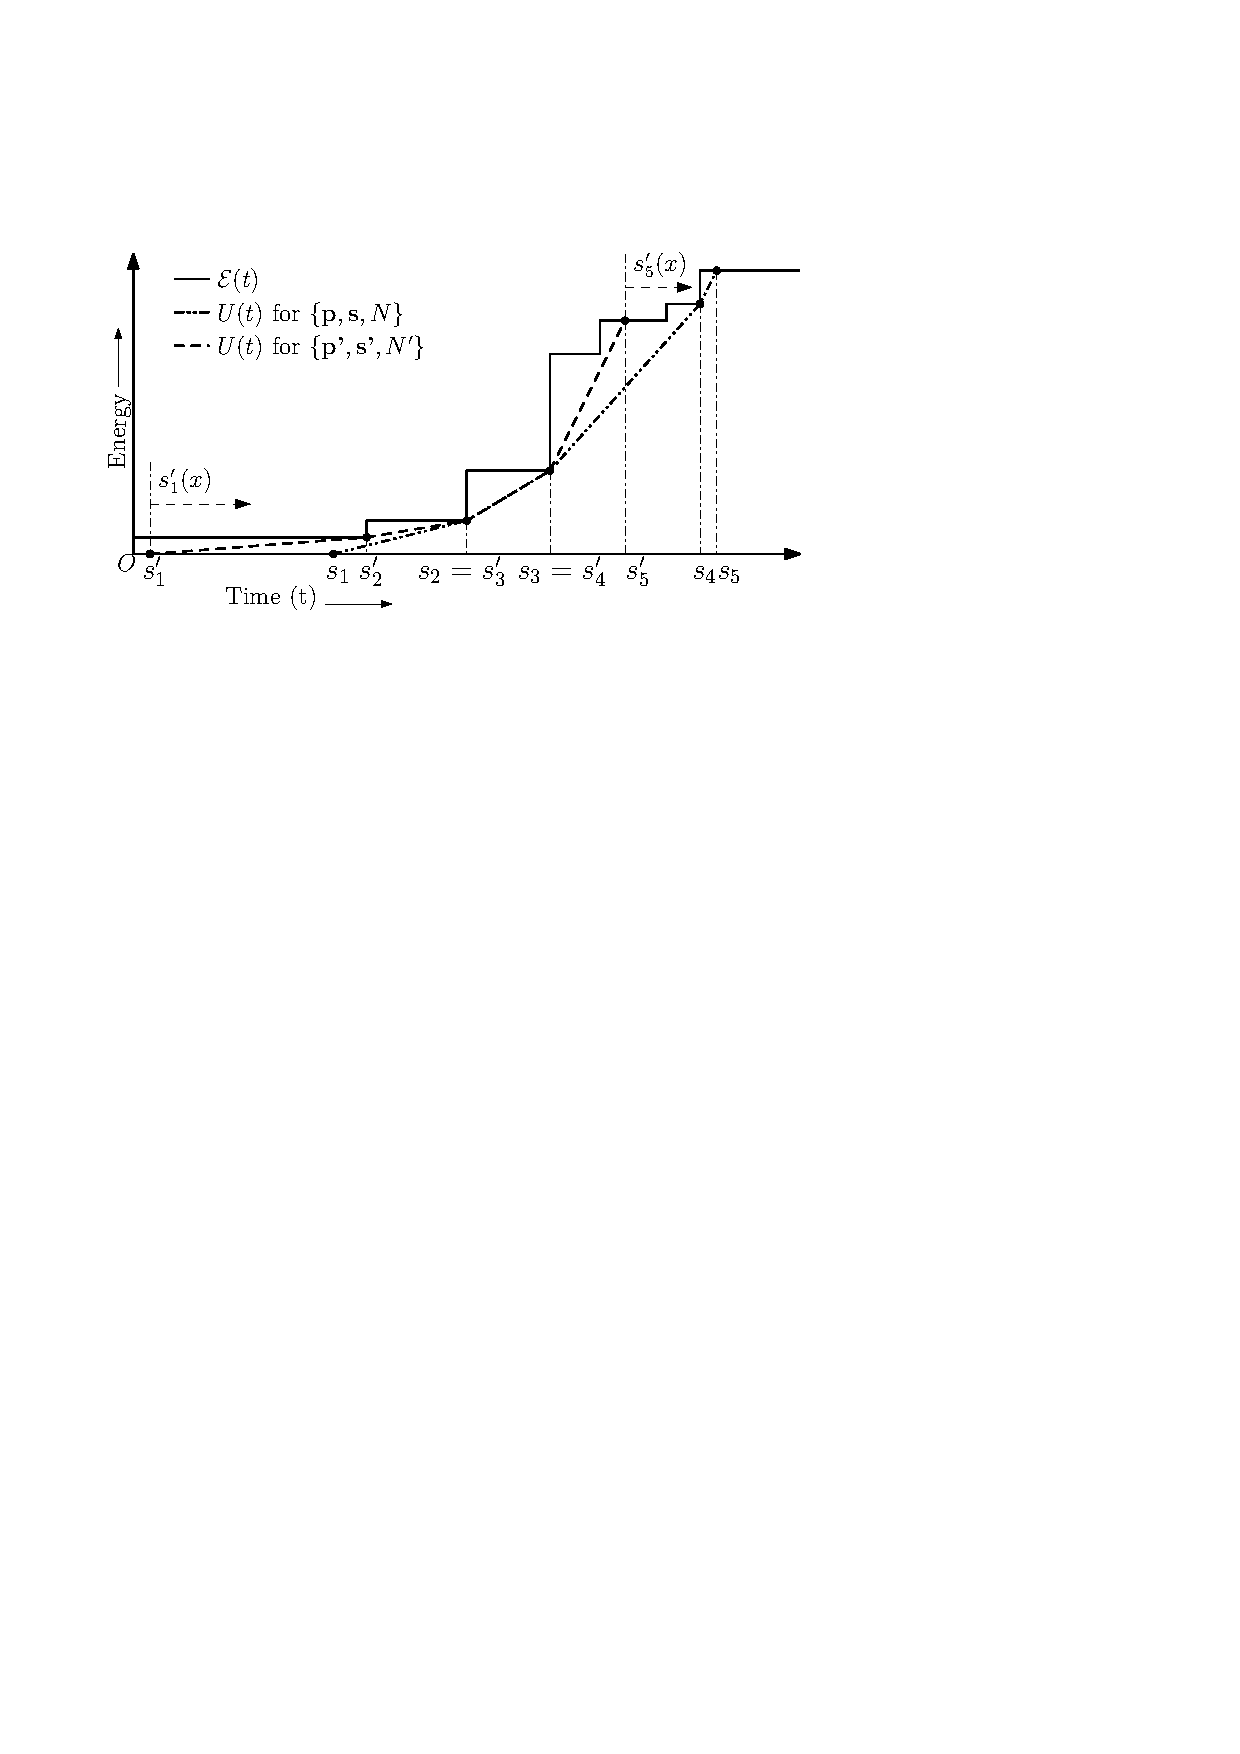
\includegraphics[width=8cm]{Theorem1_sufficient.pdf}}
\caption{Energy curves at Transmitter explaining \textit{Case3} in proof of Theorem \ref{th_algo1_1}}
\label{Theorem1_figure}
\end{figure}

Now, consider the following process which creates feasible policies from policy $\{\textbf{p'},\textbf{s'},N'\}$ as shown in Fig. \ref{Theorem1_figure}. We define two pivots $l$ and $r$. Initially we set $l=s_2'$ and $r=s_{N'}'$. The transmission power right before $l$ is $u$ ($u=p_1'$ initially) and right after $r$ is $v$ ($v=p_{N'}'$ initially). Keeping the policy same from $l$ to $r$ we increase $u$ by a small amount to $u+du$ and decrease $v$ by a small amount to $v-dv$ such that the number of bits transmitted (i.e. $B_0$) remains same under this transformation. Let $s_1'$ change to $s_1'+x$ and $s_{N'+1}'$ change to $s_{N'+1}'+y$ for some $x,y>0$ (Note that $y$ is dependent on $x$). We denote such a policy by vectors $\{\textbf{p'(x)},\textbf{s'(x)},N'(x)\}$. Following Lemma \ref{lemma_increase_time}, we can conclude that $(s_{N'(x)+1}'(x)-s_1'(x))<(s_{N'+1}'-s_1')$. We continue increasing $x$ till either $u=p_2$ (in which case we change $l=s_2$) or $v=p_{N'-1}'$ (where we change $r=s_{N'-1}'$) or $s_{N'(x)+1}'(x)$ hits an epoch, say $t_j$ ($r=t_j$, $v\rightarrow\infty$ in this case). After this, we again start increasing $x$ with changed definitions. We continue this process till $x=s_1-s_1'$  or $u$ becomes equal to $v$. Note that the former stopping criteria will be met at a smaller $x$ than the later one since policy $\{\textbf{p'(x)},\textbf{s'(x)},N'(x)\}$ shares at least one epoch with policy $X$, by arguments of previous paragraph. By maintaining these rules we ensure that policy $\{\textbf{p'(x)},\textbf{s'(x)},N'(x)\}$ abides by structure \eqref{claim1}, \eqref{claim3}-\eqref{claim5} and is feasible with energy constraint. Since $\left( s_{N'(x)+1}'(x)-s_1'(x)\right)$ is decreasing with $x$, the policy is also feasible with time constraint. As this is continuous on $x$, at $x=s_1-s_1'$ we reach a policy such that $s_1'(x)=s_1$. For $x=s_1-s_1'$, if $s_{N'(x)+1}'(x)\ge s_{N+1}$ then $s_{N'+1}'-s_1'>s_{N'(x)+1}'(x)-s_1'(x)\ge s_{N+1}-s_1=\TRx_0$ and policy $Y$ is infeasible with time constraint. If $s_{N'(x)+1}'(x)< s_{N+1}$ then we can follow the arguments in \textit{Case2} to show that policy $\{\textbf{p'(x)},\textbf{s'(x)},N'(x)\}$ is infeasible, which in turn accounts for the infeasibility of policy $Y$.
\end{proof}

























%input{Rushil}


%\begin{proof}
%To prove that the policy (say $\{\textbf{p},\textbf{s},N\}$) given by Algorithm \ref{Algorithm1} is optimal, it is sufficient to show that it abides by the structure presented in Theorem \ref{th_algo1_1}.
%
%To begin with, we prove that the power allocations in Algorithm \ref{Algorithm1} are non-decreasing. We prove this by induction. The base case constitutes of showing that, the initial feasible solution has non-decreasing powers. If INIT\_POLICY returns the constant power policy from time $R$ to $S$ with power $p_c=\frac{\ETx(t_n)}{S-R}=\frac{\ETx(t_n)-\ETx(t_q^-)}{S-t_q}$, then our claim holds. 
%
%Suppose INIT\_POLICY does not return the constant power policy, but applies Algorithm 1 from \cite{Yang} with $\widetilde{B}$ bits to transmit after time $t_q$, then the transmission power after time $t_q$ is always non-decreasing. Now, we need to prove that transmission power $p_c$ between time $R$ and $t_q$ is less than or equal to the transmission power just after time $t_q$ (say $p_i$). Let transmission with $p_i$ end at epoch $t_i$. We prove it by contradiction. Assume that $p_i<p_c$. Following two cases arise.
%
%\textit{Case1:} If $t_i<S$, energy consumed by $p_c$ between time $t_q$ to $t_i$ is 
%\begin{align}
%&p_c(t_i-t_q)>p_i(t_i-t_q)=(\ETx(t_i^-)-\ETx(t_q^-))\label{eq_1_algo1_modified}
%\end{align}
%Since, constant power policy with $p_c$ uses all the available energy by $t_q$, the maximum amount of energy available for transmission between $t_q$ and $t_i$ is $\left(\ETx(t_i^-)-\ETx(t_q^-)\right)$. But by \eqref{eq_1_algo1_modified}, $p_c$ is infeasible between time $t_q$ and $t_i$. As transmitting with power $p_c$ was feasible between $t_q$ and $S$ (and therefore between $t_q$ and $t_i$) in constant power policy, we reach a contradiction.        
%
%\textit{Case2:} If $t_i>S$, then $\ETx(t_i^-)>\ETx(S)=\ETx(t_n)$. So, 
%\begin{align}
%g(p_i)(t_i-t_q)&=g\left(\frac{\ETx(t_i^-)-\ETx(t_q^-)}{t_i-t_q}\right)(t_i-t_q)
%\\
%&>g\left(\frac{\ETx(t_n)-\ETx(t_q^-)}{t_i-t_q}\right)(t_i-t_q)
%\\
%&\stackrel{(a)}{>}g\left(\frac{\ETx(t_n)-\ETx(t_q^-)}{S-t_q}\right)(S-t_q)\label{eq_2_algo1_modified}
%\\
%&=g(p_c)(S-t_q)=\widetilde{B}.
%\end{align}
%where %\eqref{eq_2_algo1_modified} 
%$(a)$ follows from \eqref{property_decreasing}. So transmission with $p_i$ from $t_q$ to $t_i$ sends more than $\widetilde{B}$ bits. This is inconsistent with the assumption that the solution we get from Algorithm 1 in \cite{Yang} exactly transmits $\widetilde{B}$ bits after $t_q$. 
%
%Now that we have proved the base case, we assume that transmission powers from Algorithm \ref{Algorithm1} are non-decreasing till its $n^{th}$ iteration. The transmission powers between $t_l$ and $t_r$ do not change from the $n^{th}$ to the $(n+1)^{th}$ iteration, as illustrated in Fig. \ref{figure_Algorithm1}. So, we only need to prove that the transmission power before time $t_l$ is less than the transmission power after $t_l$ and the same for time $t_r$. In the $(n+1)^{th}$ iteration, by the definition of the algorithm either $t_l$ updates or $t_{r}$ updates. Assume $t_l$ gets updated to $t_{l}'$, $p_l$ to $p_l'$, $p_r$ to $p_r'$ and $t_r$ remains same. The proof for $t_r$ getting updated can be done with similar arguments and hence we only show proof of this case. If we show that $p_l<p_l'$ and $p_r>p_r'$, then we are done by induction hypothesis.
%
%If $t_l$ updates and $t_r$ remains same, then we are certain that $p_{r}'>p_r$ by algorithm definition. Now, from $n^{th}$ step to $(n+1)^{th}$ step, the number of bits transmitted after $t_r$ should decrease as $p_{r}'>p_r$. So, the number of bits transmitted before $t_l$ must be increasing from $n^{th}$ to $(n+1)^{th}$ iteration. This implies that $p_l'$ must also be less than $p_l$. In the case where $p_r$ is increased till infinity, and $t_r$ and $p_r$ are updated to their previous values, the powers must remain increasing, since $p'_l <p_l$ and the remaining powers are increasing, by the induction hypothesis. Hence we have proved that the transmission powers are always non-deceasing in the policy being output by Algorithm \ref{Algorithm1}. So it follows structure \eqref{claim3}, \eqref{claim4}.
%
%%Now, we show that transmission powers follow structure \eqref{claim3}. Assume it does not. Specifically, say $p_1$ does not follow structure \eqref{claim3}. The proof for $p_2,p_3..$ can be done likewise. So, $p_1$ has to be more than the minimum possible power i.e. $p_1>\mathcal{P}(s_1,\tilde{s})$, where $\tilde{s}=\displaystyle\argmin_{t_i: s_n < t_i \le s_{N+1}} \mathcal{P}(t_i,s_n)$. Then the amount of energy used by $p_1,p_2,..$ till epoch $\tilde{s}$ can be lower bounded by $p_1(\tilde{s}-s_1)$, as $p_1>p_2..$ . But the maximum power available till time $\tilde{s}$ is $\ETx(\tilde{s})=\mathcal{P}(s_1,\tilde{s})(\tilde{s}-s_1)>p_1(\tilde{s}-s_1)$, which is more than what is spent by $p_1$. Hence we reach a contradiction and therefore $p_1=\mathcal{P}(s_1,\tilde{s})$.
%
%Next, we show that Algorithm \ref{Algorithm1} always terminates to a policy i.e it cannot continue indefinitely. The initial policy to Algorithm \ref{Algorithm1} is given by Algorithm \ref{init_policy}. If the policy output by Algorithm \ref{init_policy}, is the constant power policy returned in line \ref{init_policy_CP}, then initially $T_{stop}-T_{start}=R-S=\widetilde{\TRx}_0$, where $\widetilde{\TRx}_0$ is defined in line \ref{init_policy_CP_time}. From line \ref{init_policy_Etn} and \ref{init_policy_CP_time} of Algorithm \ref{init_policy}, 
%\begin{align}
%& \widetilde{\TRx}_0g\left(\dfrac{\ETx(t_n)}{\widetilde{\TRx}_0}\right) = B_0, \TRx_0g\left(\dfrac{\ETx(t_n)}{\TRx_0}\right) \ge B_0.
%\end{align}    
%So $\widetilde{\TRx}_0\le \TRx_0$ by \eqref{property_decreasing}. Hence $T_{stop}-T_{start}$ is initially less or equal than $\TRx_0$.
%
%If Algorithm \ref{init_policy} returns policy from line \ref{init_policy_Yang}, then by the properties satisfied by optimal policy presented in \cite{Yang}, we know that the transmission powers would be non-decreasing after time $t_q$. The policy returned by line \ref{init_policy_Yang} is same as policy in line \ref{init_policy_CP} till time $t_q$. As transmission with power $p_c$ after $t_q$ finishes transmission of $B_0$ bits till time $S$, the policy form line \ref{init_policy_Yang}, transmitting with atleast $p_c$ or more power after $t_q$, would definitely finish before time $S$. So $T_{stop}-T_{start}$ in the initial iteration of Algorithm \ref{Algorithm1} must be less than or equal to $(R-S)=\TRx_0$. So, with policy returned by INIT\_POLICY, Algorithm \ref{Algorithm1} always enters the \textbf{while} loop in line number \ref{algo_while_loop}. From the arguments presented while proving non-decreasing powers of Algorithm \ref{Algorithm1}, we can also conclude that $T_{start}$ and $T_{stop}$ always decrease across the iterations. In all the cases of Algorithm \ref{Algorithm1}, described in Fig. \ref{figure_Algorithm1} (a) (b) (d), we can show, using Lemma \ref{lemma_increase_time}, that $T_{stop}-T_{start}$ always increases across the iterations in finite steps. So after some finite number of iterations, $T_{stop}-T_{start}$ will increase beyond $\TRx_0$, or $T_{start}$ would reach 0 and Algorithm \ref{Algorithm1} would terminate from the \textbf{while} loop in line number \ref{algo_while_loop}. Hence Algorithm \ref{Algorithm1} converges.
% 
%From the arguments presented before Theorem \ref{th_algo1_1}, we know that the policy being output by Algorithm \ref{Algorithm1} follows Lemma \ref{transmission_duration} and Lemma \ref{lemma_Q}, which imply structure \eqref{claim2} and \eqref{claim5}, respectively. To conclude, all structural results \eqref{claim1}-\eqref{claim5} are satisfied by the policy output by Algorithm \ref{Algorithm1}. Therefore,  by Theorem \ref{th_algo1_1}, Algorithm \ref{Algorithm1} results in an optimal solution.
%
%%As $T_{stop}$ decreases in every iteration of the algorithm, $t_r$ must also decrease globally, though it can increase in few iterations. Hence we can be sure that $t_r$ can potentially reach $t_q$ (Initially $t_r>t_q$). If it does reach $t_q$, then the policy    
%
%
%%      
%% 
%%First we prove that the power allocations in Algorithm \ref{Algorithm1} are in accordance with \eqref{claim3}. In any particular iteration of the algorithm, we select the maximum transmission power between $t_{l}$ and all epochs before lying in range $t_{start}$ to $t_l$. Let $t_j$ be the epoch which amounts to the maximum power and $p_j$ be the maximum power, i.e. 
%%\begin{align}
%%&t_j=\argmax_{t_i:t_{start}\le t_i< t_l} \max\left(\frac{\ETx(t_l^-)-\ETx(t_i^-)}{t_l-t_i}, \frac{\ETx(t_l^-)}{t_l-t_{start}}\right)
%%\\
%%&p_j= \max_{t_i:t_{start}\le t_i< t_l} \max\left(\frac{\ETx(t_l^-)-\ETx(t_i^-)}{t_l-t_i}, \frac{\ETx(t_l^-)}{t_l-t_{start}}\right)
%%\label{eq_max_algo1_2}
%%\end{align}
%%We claim that this is indeed the maximum over all $t_i$'s in range $s_1$ to $t_l$. To prove this by contradiction, assume that $\exists t_{a}: s_1\le t_{a}<t_{start}$ and $p_{a}=\dfrac{\ETx(t_l^-)-\ETx(t_a^-)}{t_l-t_a}>p_j $. From \eqref{eq_max_algo1_2}, we can say that 
%%\begin{align}
%%&\ETx(t_l^-)\le p_j(t_l-t_{start}),\\
%%&\implies \ETx(t_l^-)<p_a(t_l-t_{start}).
%%\end{align}
%%But transmission with power $p_a$ consumes $p_a(t_l-t_{start})$ amount of energy between $t_j$ and $t_l$, which is more than the maximum available energy till $t_l$ i.e. $\ETx(t_l^-)$. Hence transmission with $p_a$ is infeasible. 
%%
%% 
%%Now we seek to show that this procedure of selecting maximum slopes going 'backwards' also gives us the minimum slopes going 'forwards', as described in \eqref{claim3}.\\
%%We shall show this by contradiction. Let $t_i$, $t_j$ and $t_k$ be three consecutive corner points where the power of transmission increases, as per our allocation. Now suppose, it is possible to transmit with a lower power between $t_i$ and some $t'_j$. 
%%Then the power of transmission between $t_j$ and $t_k$ is not the maximum power since we could transmit at a higher power from $t'_j$ and $t_k$. Which is a contradiction as this is not consistent with out allocation algorithm.\\
%%Therefore, the allocation policy before point $t_q$ is consistent with the structure.. (See figure)
%%We can prove similarly for the powers after point $t_q$.
%\end{proof}





% !TEX root = OptimalOfflineICC.tex

%Summarising the results of Lemmas \ref{lemma_increasing_power}-\ref{transmission_duration}, the optimal policy $\{\textbf{p},\textbf{s},N\}$ may change transmission powers only at energy arrival epochs i.e. $\forall 1<i<N+1,\ s_i=t_j$ for some $j$. At these epochs, it exhausts the total energy available i.e. $U(s_i)=\ETx(s_i^-)$. The transmission powers are also non-decreasing with time and the optimal policy exhausts the total `receiver time' time allowed, if it does not start transmitting from origin.
%
%Now that we have gained some knowledge regarding the structure of the optimal policy, we consider an example to approach Problem 1. 

Using the structure of the optimal policy, we next propose an algorithm that is shown to be optimal. 

\textbf{INIT\_POLICY, Initial Feasible solution}:

\textit{Step 1}: Identify the first energy arrival instant $t_n$, so that using $\ETx(t_n)$ energy and $\TRx_0$ time, $B_0$ or more bits can be transmitted with a constant power (say $p_c$). Solve for $\widetilde{\TRx}_0$ below.
\begin{align}
&\TRx_0\left(\dfrac{\ETx(t_n)}{\TRx_0}\right)\ge B_0, \widetilde{\TRx}_0\left(\dfrac{\ETx(t_n)}{\widetilde{\TRx}_0}\right)= B_0, p_c = \dfrac{\ETx({t_n})}{\widetilde{\TRx}_0}
\label{INIT_POLICY_time}
\end{align}

\textit{Step 2}: Identify the first time instance, say $T_{start}$, such that transmission with $p_c$ for $\widetilde{\TRx}_0$ time, starting from $T_{start}$ is feasible with energy constraint \eqref{pb1_constraint_energy}. Set $T_{stop} = T_{start} + \widetilde{T}_0$. This transmission policy $p_c$, will encounter atleast one energy arrival epoch (call it $t_q$), where $U(t_q) = \ETx(t_q^-)$ (See Fig. \ref{straight}). If $U(T_{stop}) = \ETx(T_{stop}^-)$ as shown in Fig. \ref{straight}(a), then terminate with $p_c$. Otherwise, set $\widetilde{B} = (T_{stop} - t_q)g(p_c)$, which denotes the number of bits to be sent after time $t_q$. Then apply Algorithm 1 from \cite{Yang} from time $t_q$ with $\widetilde{B}$ bits to transmit (shown in Fig. \ref{straight} (b)). Update $T_{stop}$, where this policy ends. Note that, by property of Algorithm 1 from \cite{Yang}, $U(T_{stop}) = \ETx(T_{stop}^-)$.

\textbf{Algorithm 1}:

Step 3: Increase $p_r$ till $U(t_r') = \ETx(t_r'^-)$ for some $t_r'$ as shown in Fig. \ref{figure_Algorithm1}(a). If $p_r$ goes to infinity, set $p_r$ to the transmission power at $t_r^-$ and $t_r$ to the last epoch before $t_r$ where $U(t_k) = \ETx(t_k^-)$. Update $T_{stop}$ to where this policy ends. Calculate $p_l'$ such that $B_0$ bits are transmitted between $T_{stop}$ and $T_{start}'$, where $T_{start}'$ is where transmission with $p_l'$ begins.

Step 4: If $p_l'$ is feasible, which is the case shown in Fig. \ref{figure_Algorithm1}(a), set $p_l$ to $p_l'$ and $p_r$ to $p_r'$ (with $t_r$ to $t_r'$). $T_{start}$ is changed to $T_{start}'$. \textbf{GOTO} Step 3. 

Step 5: If $p_l'$ is not feasible, as shown in Fig. \ref{figure_Algorithm1}(b), then $p_l'$ is increased until it becomes feasible. $t_l'$ is set to the first instance where $U(t_l') = \ETx(t_l'^-)$ as shown in Fig. \ref{figure_Algorithm1}(c). Calculate $p_r$ such that the policy transmits $B_0$ bits. Set $t_l = t_l'$. \textbf{GOTO} Step 3.

\textbf{Termination}:

Step 6: If in any iteration at the end of Step 4 or Step 5, $T_{stop} - T_{start} = \TRx_0$ or $T_{start} = 0$, terminate.

%Suppose we are given that the receiver can be \textit{on} for a maximum duration of $\TRx_0$. Our goal is to find a transmission policy so that we can minimize the total time at which the transmission of all $B_0$ bits is completed. To do this, we shall first find a feasible solution i.e. one which satisfies all constraints (\ref{pb1_constraint_bits})-(\ref{pb1_constraint_time}) and keep improving upon it, until we have a solution that follows all structural results in Lemma \ref{lemma_increasing_power}-\ref{transmission_duration} (as shown in Theorem \ref{th_algo1_1} later,  these Lemmas form a sufficient condition as well).

We need an initial feasible solution to begin with. For this, we find the minimum energy required by the transmitter so that the transmission can be completed in duration $\TRx_0$ with a constant power. That is, the first $\ETx(t_n)$ such that
\begin{equation}
\TRx_0 g\left(\frac{\ETx(t_n)}{\TRx_0}\right)\geq B_0.
\end{equation}
Let $\widetilde{\TRx}_0\le \TRx_0$ be the time duration such that
\begin{equation}
\widetilde{\TRx}_0 g\left(\frac{\ETx(t_n)}{\widetilde{\TRx}_0}\right)=B_0.
\end{equation}
Let $p_c=\frac{\ETx(t_n)}{\widetilde{\TRx}_0}$. We try to transmit with $p_c$ power starting at time $t=0$. If it does not violate the energy constraint (\ref{pb1_constraint_energy}), we are done with the optimal solution and our transmission is completed in $\widetilde{\TRx}_0<\TRx_0$ time.

If not, we start the transmission at the earliest possible time, such that the transmission with $p_c$ for $\widetilde{\TRx}_0$ time is feasible with respect to (\ref{pb1_constraint_energy}). This transmission policy, will encounter atleast one epoch where total energy consumed till that epoch is equal to the total energy harvested upto it. Let time $t_q$ be the first point where this happens. Let $R$ and $S$ denote the starting and ending time, respectively, of transmission with power $p_c$. Clearly, $S-R=\widetilde{\TRx}_0$. This is shown in Fig. \ref{straight} (a).  Till now we have not argued why we chose such a policy to start with. In fact, Lemma \ref{lemma_Q} shows that this starting solution is a `good' estimate of policy at and before time $t_q$, as both the optimal policy and the above policy run out of all their energy at epoch $t_q$. 

Now, according to Lemma \ref{lemma_energy_consumed}, the optimal policy must finish all available energy when it stops transmission. If transmitting with $p_c$ power does use up all the energy (Fig. \ref{straight} (a)), then we accept the constant power transmission with $p_c$ as our initial policy (line number \ref{init_policy_CP} in Algorithm \ref{init_policy}). If it does not finish up all of $\ETx(t_n)$ with $p_c$ till the end of transmission (shown in Fig. \ref{straight} (b)), we choose a better policy after time $t_q$. Let $\widetilde{B}$ bits be transmitted with power $p_c$ until $S$, which is calculated in line number \ref{init_policy_bits_t_q} of procedure INIT\_POLICY in Algorithm \ref{init_policy}. Now, we require our transmission policy to send $\widetilde{B}$ bits after time $t_q$, in as little time as possible (and of course, before $S$), keeping in mind that the policy should use all $\ETx(t_n)$ amount of energy till it finishes. Algorithm 1 in \cite{Yang} does the job for us. Hence in this case, we choose transmission with $p_c$ till $t_q$ and then the solution of Algorithm 1 in \cite{Yang} after time $t_q$. 

\begin{figure}
\centering
  \centerline{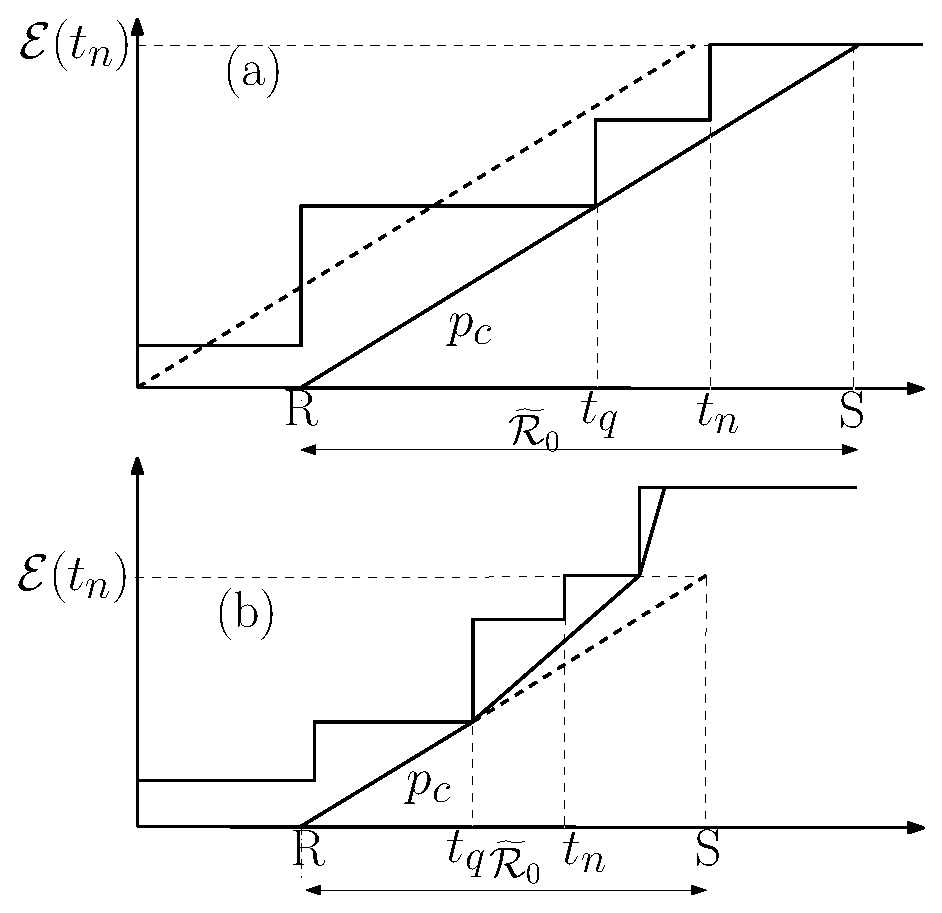
\includegraphics[width=8cm]{straight.eps}}
\caption{Figure showing point $t_q$.}\label{straight}
\end{figure}

%\begin{algorithm}
%%\algsetup{linenosize=\tiny}
%%\alglinenumber{linenosize=\scriptsize}
%\caption{Procedure to find initial feasible policy to Problem 1 for Algorithm 2}
%
%\footnotesize%\scriptsize
%\label{init_policy}
%\begin{algorithmic}[1]
%\State \textbf{Initialization}: $B_0$, $\TRx_0$
%\Procedure{INIT\_POLICY}{}
%
%\State $n=\displaystyle \argmin_k\left(\left\{t_k | \TRx_0 g\left(\frac{\ETx(t_k)}{\TRx_0}\right)\geq B_0\right\}\right)$ \label{init_policy_Etn}
%
%\State Solve for $\widetilde{T}: \widetilde{T}g\left(\dfrac{\ETx(t_n)}{\widetilde{T}}\right) = B_0$\label{init_policy_CP_time}
%
%\State $p_c=\dfrac{\ETx(n)}{\widetilde{T}}$
%
%\State $q=\displaystyle \argmin_k\ ( \{ t_k | ((\ETx(t_k) - p_ct_k) + p_ct_j) \leq \ETx(t_j),$
%
%$			 						\qquad \qquad \qquad \forall j\in[0,n]  \} )$
%\label{init_policy_t_q}
%\State $R=t_q-\dfrac{\ETx(t_q)}{p_c}$, $S=t_q+\dfrac{\ETx(t_n)-\ETx(t_q)}{p_c}$
%
%\If {$\ETx(t_n)<\ETx(S^-)$}
%	\State $\widetilde{B}=g(p_c)(S-t_q)$\label{init_policy_bits_t_q}  
%	\State $\{\textbf{p},\textbf{s},N\}\gets$  Apply Algorithm 1 in \cite{Yang} to 	minimize time of
%		\Statex   transmission of $\widetilde{B}$ bits  after time $t_q$ assuming	a  total of $\ETx_{q}$   
%		\Statex amount of energy available at $t_q$. 
%	\State\Return $\{\{p_c,\textbf{p}\},R,\textbf{s}\},N+1\}$ \label{init_policy_Yang}
%	 	\Statex (Transmission with $p_c$ from $R$ to $t_q$ and then with
%	 	\Statex policy $\{\textbf{p},\textbf{s},N\}$)
%\Else 
%	\State\Return $\{\{p_c,p_c\},\{R,t_q,S\},2\}$ \label{init_policy_CP}
%\EndIf
%\EndProcedure
%\end{algorithmic}
%\end{algorithm}



\begin{lemma}
In every optimal solution, at energy arrival epoch $t_q$, $U(t_q)=\ETx(t_q^-)$.
\label{lemma_Q}
\end{lemma}
%\begin{proof}
%We shall prove this by contradiction. First, we make the following claims:
%
%\textbf{Claim 1:} Every optimal transmission policy begins transmission at or before time $R$.
%
%Since, $S-R=\widetilde{\TRx}_0\le \TRx_0$, by Lemma \ref{transmission_duration}, if a transmission policy has to finish before $S$, it has to start before time $\max(S-\TRx_0,0) \le \max(R,0)=R$. 
%
%%Since we are transmitting all the bits at the maximum possible power, no policy that starts after $R$ can finish before $S$. Therefore, any policy that starts after $R$ cannot be optimal.
%
%\textbf{Claim 2:} Every optimal transmission policy ends transmission at or before time $S$.
%%This follows immediately from the fact that the policy is optimal.
%
%If it does not, then constant power policy $p_c$ finishing at $S$ will contradict its optimality.
%%Let $t_q$ equal to time $t_i$ for some $i\in\mathbb{N}$. 
%
%Suppose we have an optimal transmission policy, say $X$,$\{\bm{p},\bm{s},N\}$, that does not exhaust all its energy at time $t_q$ i.e. $U(t_q)<\ETx(t_q^-)$. Then, by Lemma \ref{lemma_energy_consumed}, it does not change its transmission power at $t_q$. Let the transmission power of $X$ be $p_{j-1}$ at $t_q$ and $p_{j-1}$ starts from $s_{j-1}$ and goes till $s_j$. Now, $s_j<S$ by \textit{Claim 2}. Further, power $p_c$ exhausts all energy by $t_q$. So,
%\begin{align}
%&p_c(t_q-R)=\ETx(t_q^-)\label{eqlemmaQ1}.
%\end{align}
%But, by constraint (\ref{pb1_constraint_energy}),
%\begin{align}
%&p_c(t_q-R)+p_c(s_j-t_q)\le \ETx(s_j^-),
%\\
%& p_c(s_j-t_q)\stackrel{(\ref{eqlemmaQ1})}{\le} \ETx(s_j^-)-\ETx(t_q^-),
%\\
%& p_c(s_j-t_q)< \ETx(s_j^-)-U(t_q)=p_{j-1}(s_j-t_q),
%\\
%& p_c<p_{j-1} .\label{eqlemmaQ2}
%\end{align}
%If ${j-1}= 1$, then power at $t_q$ is the first transmission power $p_1$. But then by \eqref{eqlemmaQ2}, $p_1 > p_c$. By the definition of $p_c$, we must have $s_{1} > R$, but this will contradict \textit{Claim 1}.
%
%So ${j-1}\ge 2$, which means that the power of transmission must change at least once between $R$ and $t_q$. By Lemma \ref{lemma_energy_consumed}, $X$ has used all energy by $s_{j-1}$ and $s_{j}$ as well. So, $p_{j}(\ETx(s_{j}^-)-\ETx(s_{j-1}^-))$ is the maximum energy available between time $s_{j-1}$ and $s_{j}$. If $R<s_{j-1}$, then $p_c$ (by \eqref{eqlemmaQ2}) uses more energy, than available between $s_{j-1}$ and $s_{j}$, which is not possible. If $s_{j-1}\le R$ then $p_{j-1}$ uses more than maximum energy available (given by $p_c(t_q-R)=\ETx(t_q^-)$ ) between time $R$ and $t_q$, violating energy constraint \eqref{pb1_constraint_energy}. 
%
%Therefore, every optimal transmission policy must use all energy till epoch $t_q$. 
%
%%If the optimal policy does have a power higher than $p_c$ at $t_q$, then it must have the same power of transmission either from some epoch, say $t_k$, or from the beginning of transmission. If $t_k>R$, we can show that $p_c$ becomes infeasible with respect to energy constraint (\ref{pb1_constraint_energy}) at $t_k$. If $t_k<R$, $p$ becomes infeasible with energy constraint \eqref{pb1_constraint_energy} at time $R$. Now, only thing left is the optimal policy begins transmission with power $p$. If so, then it has to begin transmission after time $R$ which follows from equation (\ref{eqlemmaQ2}). This violates \textit{Claim 1}. Therefore every optimal transmission policy must use all energy till epoch $t_q$.
%\end{proof}

Now that we have an initial feasible solution, we shall proceed to improve upon this policy as follows. The formal algorithm is presented as Algorithm \ref{Algorithm1}. We explain the procedure by an example. Assume that the starting feasible solution is given by the constant power policy, as shown by dotted line in Fig. \ref{figure_example_Algorithm1} (a), where $t_q=t_2$. We first assign the following initial values for the initial feasible policy - transmission power left of $t_2$ as $p_l=p_c$, power right of $t_2$ as $p_r=p_c$, start time $T_{start}=R$, stop time $T_{stop}=S$, epoch at which $p_l$ ends as $t_l=t_2$, epoch at which $p_r$ starts as $t_r=t_2$. Now, we increase $p_r$, keeping $t_r$ fixed, till it reaches $p_r'$ which hits epoch $t_3$, as shown by the solid line in Fig \ref{figure_example_Algorithm1} (a). As in total we need to transmit $B_0$ bits, the decrease in bits transferred by $p_r$ to $p_r'$ (RHS of \eqref{eq_example1}) is compensated by calculating appropriate $p_l'$ according to the following equation, where LHS represents the increase in bits transmitted from $p_l$ to $p_l'$.
\begin{align}
&g(p_l')\frac{\ETx(t_l^-)}{p_l'}-g(p_l)(t_l-T_{start})=-g(p_r)(T_{stop}-t_r)\nonumber\\
&+g(p_r')(\mathcal{P}(t_r,t_3))\frac{\ETx(T_{stop}^-)-ETx(t_r^-)}{\mathcal{P}(t_r,t_3)}.
\label{eq_example1}
\end{align}   
Having got a feasible $p_l'$, as shown in Fig. \ref{figure_example_Algorithm1} (a), we assign $T_{start}'$ with the point where $p_l'$ starts, $T_{stop}'$ with the point where $p_r'$ ends. $t_r'$ gets the value $t_3$ and $t_l'$ remains same as $t_l=t_2$. Note that parameters $\{T_{start}',T_{stop}',t_l',t_r',p_l',p_r'\}$ define the policy at the end of first iteration. 

In the next iteration, the portion of transmission between $t_l'=t_2$ to $t_r'=t_3$ is not updated. In this iteration, we try to increase $p_r'$ about $t_r'$ till it hits the feasibility equation \eqref{pb1_constraint_energy} of energy. $p_r'$ could virtually be increased to infinity. But transmission with infinite power for 0 time does not transmit any bits. So we assign $t_r''=t_2$ and $p_r''=\mathcal{P}(t_2,t_3)$. With this change in $p_r'$ to $p_r''$, we again calculate $p_l''$ which compensates the decrease in bits transferred after $t_r'$. But the calculated $p_l''$ becomes infeasible at $t_1$ as shown in Fig. \ref{figure_example_Algorithm1} (b). Hence, we set $p_l''$ to the maximum feasible power $\mathcal{P}(t_1,t_2)$ as shown in Fig. \ref{figure_example_Algorithm1} (c). With this $p_l''$, we re-calculate $p_r''$, so as to transmit $B_0$ bits in total. $t_l''$ is assigned to $t_1$, $t_r''$ remains $t_3$. $T_{start}''$ and $T_{stop}''$ as calculated to values marked in Fig. \ref{figure_example_Algorithm1} (c). The final policy at the end of second iteration is shown by solid line in Fig. \ref{figure_example_Algorithm1} (c). Like this, we continue to the third iteration, by improving the policy (to finish earlier) before $t_l''$ and after $t_r''$ and so on.


\begin{figure}
\centering
  \centerline{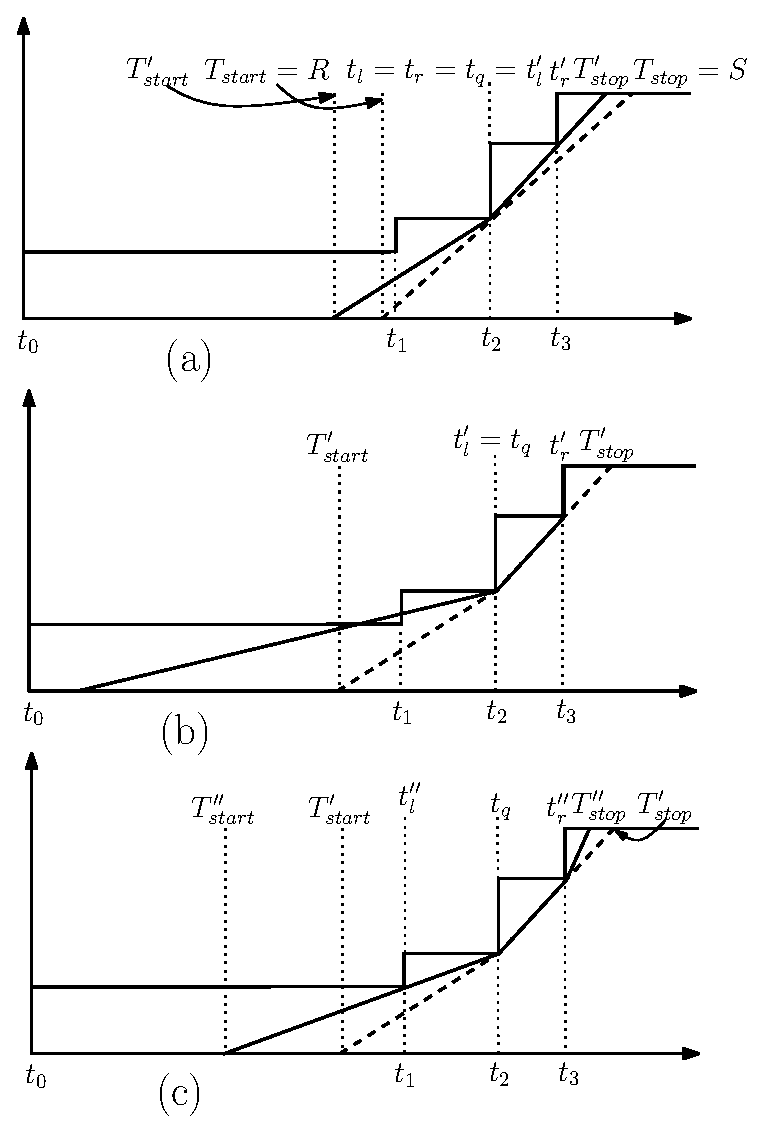
\includegraphics[width=8cm]{example_algo1.eps}}
\caption{Figures showing (a) first  and (c) second iteration of the Algorithm \ref{Algorithm1} through an example. (b) representes an intermidiate step in second iteration. In any diagram, the dashed line represent previous iteration policy and solid line is the present iteration policy.}\label{figure_example_Algorithm1}
\end{figure}


Now we describe the algorithm in steps. In any iteration, let $t_{l}$ and $t_{r}$ be the first and last energy arrival epochs where the power of transmission changes. $p_l$ and $p_r$ are the transmission power before $t_l$ and after $t_r$ respectively. $T_{start}$ and $T_{stop}$ are the start and finish time of the policy, found in any iteration. The policy found by the Algorithm in-between time $t_l$ and $t_r$ is stored in array \textbf{p} and \textbf{s}. The possible cases that can happen in an iteration of the Algorithm are shown in Fig. \ref{figure_Algorithm1}. 

Step1: The Algorithm tries to increase $p_r$ as much as possible till it hits the boundary of energy constraint \eqref{pb1_constraint_energy} as shown in Fig. \ref{figure_Algorithm1}(a). Then the Algorithm calculates the possible power $p_l'$ such that it transmits same number of bits in total with the previous iteration policy, i.e. $B_0$, as shown in line number \ref{algo_bits_left_1} and \ref{algo_bits_left_2} of Algorithm \ref{Algorithm1}. 

Step2: If $p_l'$ is feasible, which is the case shown in Fig. \ref{figure_Algorithm1}(a), the policy changes $p_l$ to $p_l'$ and $p_r$ to $p_r'$ (with $t_r$ to $t_r'$). $T_{start}$ and $T_{stop}$ are changed accordingly to start and end points of $p_l'$  and $p_r'$. 

Step3: If $p_l'$ is not feasible, as shown in Fig. \ref{figure_Algorithm1}(b), then $p_l'$ is set to be the maximum possible feasible power from $t_l$, as shown in Fig. \ref{figure_Algorithm1}(c). Now, $p_r'$ is calculated so as to settle the transmission of equal number of bits as the previous iteration. 
%We can be sure that $p_r'$ calculated now, would not be infeasible. 
In this case $t_l$ gets updated to $t_l'$.  

Going back to the first step of the algorithm where we were increasing $p_r$, it could happen, as shown in Fig. \ref{figure_Algorithm1}(d), that $p_r$ can increase to infinity without violating the energy constraint \eqref{pb1_constraint_energy}. This happens when there is no energy epoch between $t_r$ and $T_{stop}$. In this scenario, transmission is stopped at $t_r$,i.e. $T_{stop}$ gets updated to $t_r$ and both $t_r$ and $p_r$ are set to the last values in array \textbf{s},\textbf{p} receptively. This is shown in Fig. \ref{figure_Algorithm1}(d). Now, the Algorithm proceeds to calculate $p_l'$ as done in Step1, and continues as before to check whether $p_l'$ is feasible and decides according to Step2 or Step3.

\begin{figure}
\centering
  \centerline{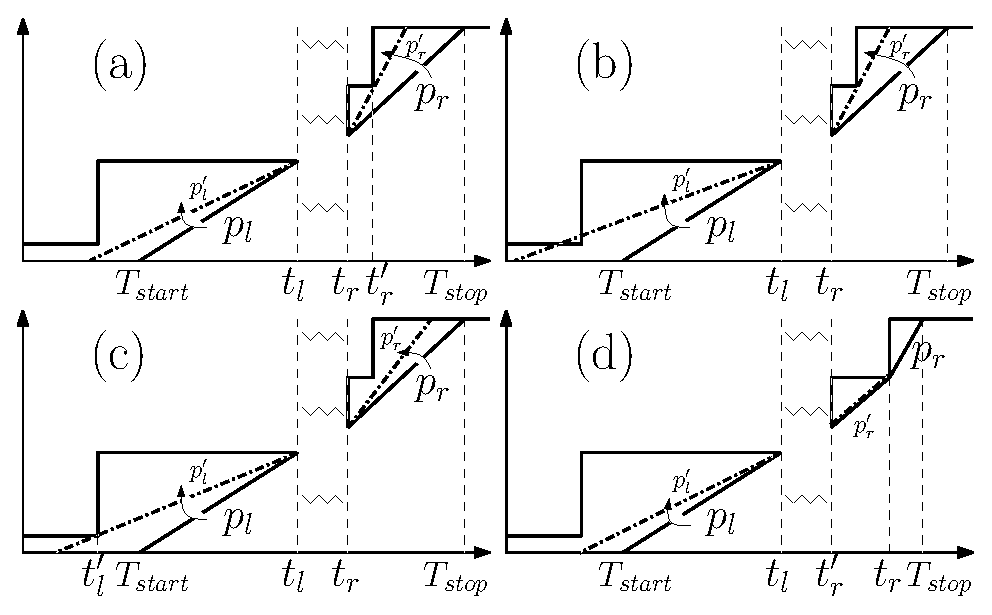
\includegraphics[width=8cm]{Algorithm1.eps}}
\caption{Figures showing any iteration of the Algorithm \ref{Algorithm1}. The solid line represents the transmission policy in the previous iteration. The dash dotted lines in (a), (b), (c), (d) represent the possible configurations of policy in the current iteration.}\label{figure_Algorithm1}
\end{figure}

This is how the algorithm proceeds to generate a new transmission policy in every iteration, which begins and ends earlier than the policy given by the previous iteration, until a point is reached where either $T_{stop}-T_{start}>\TRx_0$ or $T_{start}=0$. Suppose the Algorithm terminates with $T_{start}=0$ and $T_{start}-T_{stop}\le\TRx_0$, then the policy at this iteration is the optimal policy, as will be proved in Theorem \ref{th_algo1_2}. 


For the case where the algorithm terminates with $T_{stop}-T_{start}>\TRx_0$, let $\{T_{start}',T_{stop}',p_l',p_r',t_l',t_r'\}$ be the values in the termination iteration and $\{T_{start},T_{stop},p_l,p_r,t_l,t_r$ be the values in the previous iteration. Then, the possible valid configurations can be one of the three shown in Fig. \ref{figure_Algorithm1} (a) (c) (d). Note that $\ETx(T_{stop}^-)=\ETx(T_{stop}'^-)$ in all the cases. (In case Fig. \ref{figure_Algorithm1} (d) we can assume that $T_{stop}'=t_r^+$ and transmission exists after $t_r$, but with infinite power. Since transmitting with infinite power for $0$ time does not transmit any bits, we would transmit the same number of bits, as we did prior to this modification). Thus, by Lemma \ref{lemma_increase_time}, we can verify that $(T_{stop}'-T_{start}')>(T_{stop}-T_{start})$. Since $(T_{stop}'-T_{start}')>\TRx_0>(T_{stop}-T_{start})$, there must exist a solution to equation presented in line number \ref{algo_solve_eqn} of Algorithm \ref{Algorithm1}. Let the policy obtained from the solution start and end at $T_{start}''$ and $T_{stop}''$. Then $T_{stop}''$ and $T_{start}''$ would lie in-between $T_{stop}$,$T_{stop}'$ and $T_{start}$,$T_{start}'$ respectively. Also, $T_{stop}''-T_{start}''=\TRx_0$.




So we can conclude by stating that, the solution to Algorithm \ref{Algorithm1} satisfies Lemma \ref{transmission_duration}. Now, according to the definition of $t_n$ and $t_q$ in line number \ref{init_policy_Etn} and \ref{init_policy_t_q} of INIT\_POLICY, $t_q\le t_n$ and $\ETx(t_q)<\ETx(t_n)$. Since $t_n$ is defined as the first energy arrival epoch by which $B_0$ bits can be transmitted in $\TRx_0$ time, any transmission policy which ends at or before $t_n$ should take more than $\TRx_0$ time to transmit all of $B_0$ bits. As $t_q\le t_n$, we are guaranteed that no transmission policy can finish at or before $t_q$. Hence in the iterations of the algorithm $t_r$ can never decrease beyond $t_q$. As $t_q$ is present in the initial solution, $t_q$ always exists in the final solution to Algorithm \ref{Algorithm1}.   
\begin{theorem}
A transmission policy $\{\textbf{p},\textbf{s},N\}$ is an optimal solution to Problem 1 if and only if it satisfies the following structure.
\label{th_algo1_1}
\begin{align}
&\sum_{i=1}^{i=N}g(p_i)(s_{i+1}-s_i)=B_0; 								
\label{claim1}
\\
&p_1\le p_2 ..\le p_N;
\label{claim3}  
\\
&\nonumber s_i=t_j \text{ for some } j, i\in \{2,..,N\} \ \text{ and }
\\
& U(s_i)=\ETx(s_i^-), \forall i\in \{2,..,N+1\};
\label{claim4}
\\
&\nonumber s_{N+1}-s_1=\mathcal{R}_0, 	 \ \ \ \ 						\text{ if } s_1>0 \text{ or }
\\
& s_{N+1}\le \mathcal{R}_0,				\ \ \ \ \ \ \ \ \ \				\text{ if } s_1=0;
\label{claim2}
\\
&\exists s_j:s_j\in \textbf{s} \text{ and } s_j=t_q.
\label{claim5}
\end{align}
%& \nonumber s_{n+1}=\argmin_{t_i: s_n < t_i \le s_{N+1}} \mathcal{P}(s_n,t_i)=\dfrac{\ETx(t_i^-)-U(s_n)}{t_i-s_n} \	\text{ and }
%\\
%&p_n=\mathcal{P}(s_{n},s_{n+1});\label{claim3}							
%\\
\end{theorem}

\begin{theorem}
The proposed transmission policy is an optimal solution to Problem 1.
\label{th_algo1_2}
\end{theorem}
\begin{proof}
To prove that the policy (say $\{\textbf{p},\textbf{s},N\}$) given by Algorithm \ref{Algorithm1} is optimal, it is sufficient to show that it abides by the structure presented in Theorem \ref{th_algo1_1}.

To begin with, we prove that the power allocations in Algorithm \ref{Algorithm1} are non-decreasing. We prove this by induction. The base case constitutes of showing that, the initial feasible solution has non-decreasing powers. If INIT\_POLICY returns the constant power policy from time $R$ to $S$ with power $p_c=\frac{\ETx(t_n)}{S-R}=\frac{\ETx(t_n)-\ETx(t_q^-)}{S-t_q}$, then our claim holds. 

Suppose INIT\_POLICY does not return the constant power policy, but applies Algorithm 1 from \cite{Yang} with $\widetilde{B}$ bits to transmit after time $t_q$, then the transmission power after time $t_q$ is always non-decreasing. Now, we need to prove that transmission power $p_c$ between time $R$ and $t_q$ is less than or equal to the transmission power just after time $t_q$ (say $p_i$). Let transmission with $p_i$ end at epoch $t_i$. We prove it by contradiction. Assume that $p_i<p_c$. Following two cases arise.

\textit{Case1:} If $t_i<S$, energy consumed by $p_c$ between time $t_q$ to $t_i$ is 
\begin{align}
&p_c(t_i-t_q)>p_i(t_i-t_q)=(\ETx(t_i^-)-\ETx(t_q^-))\label{eq_1_algo1_modified}
\end{align}
Since, constant power policy with $p_c$ uses all the available energy by $t_q$, the maximum amount of energy available for transmission between $t_q$ and $t_i$ is $\left(\ETx(t_i^-)-\ETx(t_q^-)\right)$. But by \eqref{eq_1_algo1_modified}, $p_c$ is infeasible between time $t_q$ and $t_i$. As transmitting with power $p_c$ was feasible between $t_q$ and $S$ (and therefore between $t_q$ and $t_i$) in constant power policy, we reach a contradiction.        

\textit{Case2:} If $t_i>S$, then $\ETx(t_i^-)>\ETx(S)=\ETx(t_n)$. So, 
\begin{align}
g(p_i)(t_i-t_q)&=g\left(\frac{\ETx(t_i^-)-\ETx(t_q^-)}{t_i-t_q}\right)(t_i-t_q)
\\
&>g\left(\frac{\ETx(t_n)-\ETx(t_q^-)}{t_i-t_q}\right)(t_i-t_q)
\\
&\stackrel{(a)}{>}g\left(\frac{\ETx(t_n)-\ETx(t_q^-)}{S-t_q}\right)(S-t_q)\label{eq_2_algo1_modified}
\\
&=g(p_c)(S-t_q)=\widetilde{B}.
\end{align}
where %\eqref{eq_2_algo1_modified} 
$(a)$ follows from \eqref{property_decreasing}. So transmission with $p_i$ from $t_q$ to $t_i$ sends more than $\widetilde{B}$ bits. This is inconsistent with the assumption that the solution we get from Algorithm 1 in \cite{Yang} exactly transmits $\widetilde{B}$ bits after $t_q$. 

Now that we have proved the base case, we assume that transmission powers from Algorithm \ref{Algorithm1} are non-decreasing till its $n^{th}$ iteration. The transmission powers between $t_l$ and $t_r$ do not change from the $n^{th}$ to the $(n+1)^{th}$ iteration, as illustrated in Fig. \ref{figure_Algorithm1}. So, we only need to prove that the transmission power before time $t_l$ is less than the transmission power after $t_l$ and the same for time $t_r$. In the $(n+1)^{th}$ iteration, by the definition of the algorithm either $t_l$ updates or $t_{r}$ updates. Assume $t_l$ gets updated to $t_{l}'$, $p_l$ to $p_l'$, $p_r$ to $p_r'$ and $t_r$ remains same. The proof for $t_r$ getting updated can be done with similar arguments and hence we only show proof of this case. If we show that $p_l<p_l'$ and $p_r>p_r'$, then we are done by induction hypothesis.

If $t_l$ updates and $t_r$ remains same, then we are certain that $p_{r}'>p_r$ by algorithm definition. Now, from $n^{th}$ step to $(n+1)^{th}$ step, the number of bits transmitted after $t_r$ should decrease as $p_{r}'>p_r$. So, the number of bits transmitted before $t_l$ must be increasing from $n^{th}$ to $(n+1)^{th}$ iteration. This implies that $p_l'$ must also be less than $p_l$. In the case where $p_r$ is increased till infinity, and $t_r$ and $p_r$ are updated to their previous values, the powers must remain increasing, since $p'_l <p_l$ and the remaining powers are increasing, by the induction hypothesis. Hence we have proved that the transmission powers are always non-deceasing in the policy being output by Algorithm \ref{Algorithm1}. So it follows structure \eqref{claim3}, \eqref{claim4}.

%Now, we show that transmission powers follow structure \eqref{claim3}. Assume it does not. Specifically, say $p_1$ does not follow structure \eqref{claim3}. The proof for $p_2,p_3..$ can be done likewise. So, $p_1$ has to be more than the minimum possible power i.e. $p_1>\mathcal{P}(s_1,\tilde{s})$, where $\tilde{s}=\displaystyle\argmin_{t_i: s_n < t_i \le s_{N+1}} \mathcal{P}(t_i,s_n)$. Then the amount of energy used by $p_1,p_2,..$ till epoch $\tilde{s}$ can be lower bounded by $p_1(\tilde{s}-s_1)$, as $p_1>p_2..$ . But the maximum power available till time $\tilde{s}$ is $\ETx(\tilde{s})=\mathcal{P}(s_1,\tilde{s})(\tilde{s}-s_1)>p_1(\tilde{s}-s_1)$, which is more than what is spent by $p_1$. Hence we reach a contradiction and therefore $p_1=\mathcal{P}(s_1,\tilde{s})$.

Next, we show that Algorithm \ref{Algorithm1} always terminates to a policy i.e it cannot continue indefinitely. If the policy output by INIT\_POLICY, is the constant power policy $p_c$, then initially $T_{stop}-T_{start}=\widetilde{\TRx}_0$, where $\widetilde{\TRx}_0$ is defined in line \ref{init_policy_CP_time}. From line \ref{init_policy_Etn} and \ref{init_policy_CP_time} of Algorithm \ref{init_policy}, 
\begin{align}
& \widetilde{\TRx}_0g\left(\dfrac{\ETx(t_n)}{\widetilde{\TRx}_0}\right) = B_0, \TRx_0g\left(\dfrac{\ETx(t_n)}{\TRx_0}\right) \ge B_0.
\end{align}    
So $\widetilde{\TRx}_0\le \TRx_0$ by \eqref{property_decreasing}. Hence $T_{stop}-T_{start}$ is initially less or equal than $\TRx_0$.

If Algorithm \ref{init_policy} returns policy from line \ref{init_policy_Yang}, then by the properties satisfied by optimal policy presented in \cite{Yang}, we know that the transmission powers would be non-decreasing after time $t_q$. The policy returned by line \ref{init_policy_Yang} is same as policy in line \ref{init_policy_CP} till time $t_q$. As transmission with power $p_c$ after $t_q$ finishes transmission of $B_0$ bits till time $S$, the policy form line \ref{init_policy_Yang}, transmitting with atleast $p_c$ or more power after $t_q$, would definitely finish before time $S$. So $T_{stop}-T_{start}$ in the initial iteration of Algorithm \ref{Algorithm1} must be less than or equal to $(R-S)=\TRx_0$. So, with policy returned by INIT\_POLICY, Algorithm \ref{Algorithm1} always enters the \textbf{while} loop in line number \ref{algo_while_loop}. From the arguments presented while proving non-decreasing powers of Algorithm \ref{Algorithm1}, we can also conclude that $T_{start}$ and $T_{stop}$ always decrease across the iterations. In all the cases of Algorithm \ref{Algorithm1}, described in Fig. \ref{figure_Algorithm1} (a) (b) (d), we can show, using Lemma \ref{lemma_increase_time}, that $T_{stop}-T_{start}$ always increases across the iterations in finite steps. So after some finite number of iterations, $T_{stop}-T_{start}$ will increase beyond $\TRx_0$, or $T_{start}$ would reach 0 and Algorithm \ref{Algorithm1} would terminate from the \textbf{while} loop in line number \ref{algo_while_loop}. Hence Algorithm \ref{Algorithm1} converges.
 
From the arguments presented before Theorem \ref{th_algo1_1}, we know that the policy being output by Algorithm \ref{Algorithm1} follows Lemma \ref{transmission_duration} and Lemma \ref{lemma_Q}, which imply structure \eqref{claim2} and \eqref{claim5}, respectively. To conclude, all structural results \eqref{claim1}-\eqref{claim5} are satisfied by the policy output by Algorithm \ref{Algorithm1}. Therefore,  by Theorem \ref{th_algo1_1}, Algorithm \ref{Algorithm1} results in an optimal solution.
\end{proof}




\section{ONLINE ALGORITHM FOR ENERGY HARVESTING TRANSMITTER AND RECEIVER}
% !TEX root = ICC.tex
In an online scenario, transmitter and receiver are assumed to have only causal information about energy arrivals i.e. they have no knowledge of future energy harvests. To model a general energy harvesting system, they are further assumed to not have any information about the distribution of future energy arrivals. We propose an algorithm to schedule the transmission of bits in this model. Motivated by \cite{VazeCompetitive}, we use competitive ratio analysis to compare the performance of online policy vs. the optimal offline policy. In this context, we say that our algorithm is $r$-competitive if for all possible energy arrivals at the transmitter $\ETx(t)$ and all possible `time' arrival $\TRx(t)$ at the receiver, the ratio of time taken by the online algorithm (say $T_{\mbox{\scriptsize{online}}}$) to the optimal offline one (say $T_{\mbox{\scriptsize{off}}}$) is bounded by $r$.
\begin{align}
&\displaystyle\max_{\ETx(t),\TRx(t)\hspace{0.5mm} \forall t}\dfrac{T_{\mbox{\scriptsize{online}}}}{T_{\mbox{\scriptsize{off}}}}\le r.
\end{align}
 
\textit{Notation:} The starting time of transmission is denoted by $T_{\mbox{\scriptsize{start}}}$ and the present time is denoted by $t$. The number of bits and energy remaining to transmit at any transmitter energy epoch is represented by $B_{\mbox{\scriptsize{rem}}}$ and $E_{\mbox{\scriptsize{rem}}}$ receptively. We use the same notation $\{\bm{p},\bm{s},N\}$ to denote an onilne policy as described for offline policies.

%The online algorithm that we propose is presented in Algorithm \ref{algo_online}. 
\textit{Online Algorithm:} The Algorithm waits till time $T_{\mbox{\scriptsize{start}}}$ which marks the first energy arrival at transmitter or `time' addition at receiver such that using the energy $\ETx(T_{\mbox{\scriptsize{start}}})$ and time $\TRx(T_{\mbox{\scriptsize{start}}})$, $B_0$ or more bits can be transmitted.
\begin{equation}
T_{\mbox{\scriptsize{start}}}=\min\ t \ s.t.\  \TRx(t)g\Bigg{(} \dfrac{\ETx(t)}{\TRx(t)}\Bigg{)}\ge B_0.\label{online_T_start}
\end{equation}

To begin with, the transmitter equally divides $\ETx(T_{\mbox{\scriptsize{start}}})$ energy among all $B_0$ bits i.e. the first transmission power $p_1$ is set such that,
\begin{align}
&\frac{\ETx(T_{\mbox{\scriptsize{start}}})}{p_1}g(p_1)=B_0.
\label{eq_online_first_power}
\end{align}

By definition of $T_{\mbox{\scriptsize{start}}}$ in \eqref{online_T_start}, we know that transmission with power $p_1$ is going to finish in less than or equal to  $\TRx(T_{\mbox{\scriptsize{start}}})$ time.

If and when energy is harvested at the transmitter, the transmission power is changed. The total unused energy left at such an instant, $E_{\mbox{\scriptsize{rem}}}$, is equally divided among the bits left to transmit, $B_{\mbox{\scriptsize{rem}}}$ i.e. 
\begin{equation}
\frac{E_{\mbox{\scriptsize{rem}}}}{p} g(p)= B_{\mbox{\scriptsize{rem}}}.\end{equation}
Note that we do not change our transmission power when there is a `time' arrival at the receiver after $T_{\mbox{\scriptsize{start}}}$, because there is sufficient receiver time already available to finish transmission. Also, the online algorithm changes its transmission power at every transmitter energy epoch after $T_{\mbox{\scriptsize{start}}}$ unlike the optimal offline policy. 

\textit{Example:} Fig. \ref{figure_online_example} shows output of online algorithm, for certain $\ETx(t)$ and $\TRx(t)$. Initially, suppose $B_0$ bits are not possible to be sent with $\ETx_0$ energy  within $\TRx_0$ time i.e. $\TRx(t_0)g\left( \dfrac{\ETx(t_0)}{\TRx(t_0)}\right)<B_0$. Further, $\TRx(r_1)g\left( \dfrac{\ETx(r_1)}{\TRx(r_1)}\right)<B_0$ and $\TRx(t_1)g\left( \dfrac{\ETx(t_1)}{\TRx(t_1)}\right)<B_0$. But, $\TRx(r_2)g\left( \dfrac{\ETx(r_2)}{\TRx(r_2)}\right)>B_0$. So, transmitter starts its transmission at $T_{\mbox{\scriptsize{start}}}=r_2$ with a power $p_1$ such that at rate $g(p_1)$, $B_0$ bits can be sent in $\ETx(r_2)/p_1$ time, as given in \eqref{eq_online_first_power}. At time $t=r_2$, transmitter expects transmission to finish by $r_2+\ETx(r_2)/p_1$ time. But, due to new energy arrival at time $t_2$, it can finish transmission earlier at a higher rate than $p_1$. At $t=t_2$, energy stored at transmitter is $E_{\mbox{\scriptsize{rem}}}=\ETx(r_2)+\ETx_2-(t_2-r_2)p_1$ and bits left to transmit is $B_{\mbox{\scriptsize{rem}}}=B_0-(t_2-r_2)g(p_1)$. Transmission power changes to $p_2$ at time $t_2$ such that $\frac{E_{\mbox{\scriptsize{rem}}}}{p_2}g(p_2)=B_{\mbox{\scriptsize{rem}}}$. Due to no new energy arrival till time $t_2+\frac{E_{\mbox{\scriptsize{rem}}}}{p_2}$, transmission completes at rate $p_2$, sending $B_0$ bits. 

\begin{figure}
\centering
  \centerline{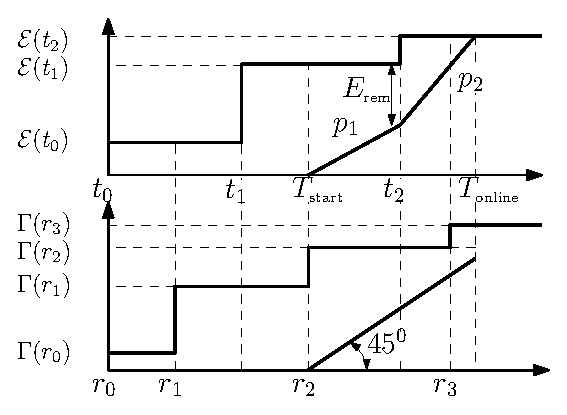
\includegraphics[width=8cm]{online.eps}}
\caption{Example showing execution of the online algorithm. The value of $E_{\mbox{\scriptsize{rem}}}$ is marked at time $t_2$.}\label{figure_online_example}
\end{figure}


%\begin{algorithm}
%\caption {On-line Algorithm for energy harvesting transmitter and receiver.}
%\footnotesize
%\label{algo_online}
%\begin{algorithmic}[1]
%\State \textbf{Input}: Bits to transmit $B_0$; $\ETx_i$, $\TRx_i$ for $t_i,r_i<t$ where $t$ is the present time instant which increments parallely with this algorithm. 
%
%\State $T_{\mbox{\scriptsize{start}}}=\min\ t$ s.t. $\TRx(t)g\Bigg{(} \dfrac{\ETx(t)}{\TRx(t)}\Bigg{)}\ge B_0$
%\State $B_{\mbox{\scriptsize{rem}}}=B_0$, $E_{\mbox{\scriptsize{rem}}}=\ETx(T_{\mbox{\scriptsize{start}}})$, $m=T_{\mbox{\scriptsize{start}}}$
%
%\Do
%	\State Transmit at power $p$ such that $\dfrac{E_{\mbox{\scriptsize{rem}}}}{p} g(p)= B_{\mbox{\scriptsize{rem}}}$
%	\If {$t=t_i$ for some $i$} 
%		\State $B_{\mbox{\scriptsize{rem}}}=B_{\mbox{\scriptsize{rem}}}-(t_i-m)g(p)$
%		\State $E_{\mbox{\scriptsize{rem}}}=E_{\mbox{\scriptsize{rem}}}+\ETx_i-(t_i-m)p$
%		\State $m=t_i$
%	\EndIf
%\DoWhile {$t\le \left( m+\dfrac{E_{\mbox{\scriptsize{rem}}}}{p}\right)$}
%\end{algorithmic}
%\end{algorithm}

\begin{lemma}
The transmission power in the on-line algorithm is non-decreasing with time.
\label{online_power}
\end{lemma}
%\begin{proof}
%From the definition of the algorithm, the transmission power only changes at energy arrival in transmitter, after $T_{\mbox{\scriptsize{start}}}$. 
%
%Suppose there are energy arrivals after $T_{\mbox{\scriptsize{start}}}$ and for any energy arrival (say $E_{\mbox{\scriptsize{new}}}$) the power changes from $p_i$ to $p_{i+1}$. Let the energy remaining at start of transmission with power $p_i$ be $E_{\mbox{\scriptsize{rem}}}$ and bits remaining be $B_{\mbox{\scriptsize{rem}}}$. The transmission continues for time $l_i$ with power $p_i$. Now, we need to show that $p_i<p_{i+1}$. From the algorithm we get the following equations.  
%\begin{align}
%&\frac{g(p_i)}{p_i}=\frac{B_{\mbox{\scriptsize{rem}}}}{E_{\mbox{\scriptsize{rem}}}} \label{power_increasing_eq1},
%\\
%&\frac{g(p_{i+1})}{p_{i+1}}=\frac{B_{\mbox{\scriptsize{rem}}}-g(p_i) l_i}{E_{\mbox{\scriptsize{rem}}}+E_{\mbox{\scriptsize{new}}}-p_i l_i}.\label{power_increasing_eq2}
%\end{align}
%
%Substituting $g(p_i)$ from (\ref{power_increasing_eq1}) into RHS of (\ref{power_increasing_eq2}), we can see that $\frac{g(p_i)}{p_i}>\frac{g(p_{i+1})}{p_{i+1}}$. Hence, by monotonicity of $g(p)/p$ from \eqref{property_decreasing}, we know that $p_i<p_{i+1}$.
%\end{proof}

\begin{lemma}
In the online policy, if the transmission power at time $t$ is $p$, then $\dfrac{\ETx(t)}{{p}}g(p) \le B_0\;\;\forall\;\; t\in [T_{\mbox{\scriptsize{start}}}, T_{\mbox{\scriptsize{online}}}]$ with equality at $t=T_{\mbox{\scriptsize{start}}}$.
\label{lemma_online_inequality}
\end{lemma}


%\begin{lemma}
%In the online policy $\{\bm{p},\bm{s},N\}$, $\dfrac{g(p_i)}{p_i}\le \dfrac{B_0}{\ETx(s_i)}$.
%\label{lemma_online_inequality}
%\end{lemma}


\begin{proof}
Suppose the online policy is denoted by $\{\bm{p},\bm{s},N\}$. It is then enough to prove that $\frac{g(p_i)}{p_i} \le \frac{B_0}{\ETx(s_i)}$ for $i\in\{1,..,N\} $, because both $p_i$ and $\ETx(t)$ remains constant in $t\in[s_i,s_{i+1})$. We prove it by induction on $i$ in ordered set $\{1,2..,N\}$. 

With $s_1=T_{\mbox{\scriptsize{start}}}$, the base case follows form equality \eqref{eq_online_first_power}. Now, assume $\frac{g(p_i)}{p_i}\le \frac{B_0}{\ETx(s_i)}$ to be true for $i=k-1$, $k\in \{2,..,N\}$. Let $E_{\mbox{\scriptsize{rem}}}$ and $B_{\mbox{\scriptsize{rem}}}$ be the residual energy and bits, at time $s_{k-1}$. As $s_k=t_j$ for some $j$, we can write,
\begin{align*}
&\frac{p_{k}}{g(p_{k})}=\frac{E_{\mbox{\scriptsize{rem}}}+E_{j}-p_{k-1} (s_k-s_{k-1})}{B_{\mbox{\scriptsize{rem}}}-g(p_{k-1}) (s_k-s_{k-1})},
\\
&\stackrel{(a)}{=}\frac{p_{k-1}}{g(p_{k-1})}+\frac{E_{j}}{B_{\mbox{\scriptsize{rem}}}\gamma}
\stackrel{(b)}{>}\frac{\ETx(s_{k-1})}{B_0}+\frac{E_{j}}{B_0}=\frac{{\ETx(s_{k})}}{B_0}.
\end{align*}

where $(a)$ follows form $\frac{B_{\mbox{\scriptsize{rem}}}}{E_{\mbox{\scriptsize{rem}}}}=\frac{g(p_{k-1})}{p_{k-1}}$ and substitution $\gamma=\left( 1-\frac{p_{k-1}}{E_{\mbox{\scriptsize{rem}}}} (s_k-s_{k-1})\right)< 1$;  $(b)$ uses induction hypothesis along with the inequality $B_{\mbox{\scriptsize{rem}}}\gamma< B_0$. This completes the proof of Lemma \ref{lemma_online_inequality}. From equality $(a)$ we can see that $g(p_k)/p_k<g(p_{k-1})/p_{k-1}$. Hence, by monotonicity of $g(p)/p$, $p_{k}>p_{k-1}$. This proofs Lemma \ref{online_power}.
\end{proof}



\begin{lemma}
The online policy starts atleast by the time the optimal offline policy ends i.e. $T_{\mbox{\scriptsize{start}}} <T_{\mbox{\scriptsize{off}}}$.
\label{onilne_time}
\end{lemma}


\begin{proof}
We will prove this by contradiction. Suppose $T_{\mbox{\scriptsize{start}}} \ge T_{\mbox{\scriptsize{off}}}$. From \eqref{online_T_start}, either $T_{\mbox{\scriptsize{start}}}=t_i$ for some $i$ and/or $T_{\mbox{\scriptsize{start}}}=r_j$ for some $j$.

If $T_{\mbox{\scriptsize{start}}}=t_i$, then %as $T_{\mbox{\scriptsize{off}}}\le T_{\mbox{\scriptsize{start}}}$, 
the maximum energy that can be utilized by the offline policy is $\ETx(T_{\mbox{\scriptsize{start}}}^-)=\TRx(T_{\mbox{\scriptsize{start}}})-\ETx_i\neq \TRx(T_{\mbox{\scriptsize{start}}})$.
%Note that the offline policy cannot use energy arrival $\ETx_i$, as using any finite amount of energy for 0 time cannot deliver any bits. 

If $T_{\mbox{\scriptsize{start}}}=r_j$, then the maximum time for which the receiver can be \textit{on} in the offline policy is $\TRx(T_{\mbox{\scriptsize{start}}}^-)=\TRx(T_{\mbox{\scriptsize{start}}})-\TRx_j\neq \TRx(T_{\mbox{\scriptsize{start}}})$.
%, as the offline policy has to finish at or before $T_{\mbox{\scriptsize{start}}}$. 
%Note that, in the optimal offline policy, time for which the receiver is \textit{on} is given by $\displaystyle \sum_{i:p_i\neq 0}(s_{i+1}-s_i)$. 

%If $T_{\mbox{\scriptsize{start}}}\neq t_i$ or $T_{\mbox{\scriptsize{start}}}\neq r_j$ then, $\ETx(T_{\mbox{\scriptsize{start}}}^-)=\ETx(T_{\mbox{\scriptsize{start}}})$ or $\TRx(T_{\mbox{\scriptsize{start}}}^-)=\TRx(T_{\mbox{\scriptsize{start}}})$.

Now, the number of bits transmitted by the offline policy $\{\bm{p},\bm{s},N\}$ is given by,
\begin{align}
&\sum_{{\substack{i=1\\p_i\neq 0}}}^{i=N} g(p_i)(s_{i+1}-s_{i}),
\\
&\nonumber \stackrel{(a)}{\le}g\left(\frac{\displaystyle\sum_{i:p_i\neq 0}p_i(s_{i+1}-s_{i})}{\displaystyle\sum_{j:p_j\neq 0}(s_{j+1}-s_{j})}\right)\sum_{j:p_j\neq 0} (s_{j+1}-s_{j}),
\\
&\stackrel{(b)}\le g\left(\frac{\ETx(T_{\mbox{\scriptsize{start}}}^-)}{\TRx(T_{\mbox{\scriptsize{start}}}^-)}\right)\TRx(T_{\mbox{\scriptsize{start}}}^-)\stackrel{(c)}{<}B_0.\label{online_eq_2}
\end{align}
%%%&\nonumber\stackrel{(b)}{\le} g\left( \frac{\displaystyle\sum_{i:p_i\neq 0} p_i(s_{i+1}-s_{i})}{\TRx(T_{\mbox{\scriptsize{start}}}^-)} \right)\TRx(T_{\mbox{\scriptsize{start}}}^-), 
%%%&\nonumber\stackrel{(a)}{\le} g\left(\sum_{\substack{i\\p_i\neq 0}}p_i\left(\frac{(s_{i+1}-s_{i})}{\displaystyle\sum_{j:p_j\neq 0}(s_{j+1}-s_{j})}\right)\right) \sum_{\substack{j\\p_j\neq 0}} (s_{j+1}-s_{j}),

where $(a)$ follows from application of Jensen's inequality due to concavity of $g(p)$; $(b)$ follows form the fact that $\displaystyle\sum_{j:p_j\neq 0}(s_{j+1}-s_{j})\le\TRx(T_{\mbox{\scriptsize{off}}})\le \TRx(T_{\mbox{\scriptsize{start}}}^-)$ and $g(p)/p$ is monotonically decreasing; $(c)$ follows form \eqref{online_T_start}. \eqref{online_eq_2} implies that the number of bits transmitted by the offline policy is less than $B_0$. Therefore, by contradiction, $T_{\mbox{\scriptsize{start}}}<T_{\mbox{\scriptsize{off}}}$.
\end{proof}



\begin{theorem}
The competitive ratio of the online policy is strictly less than 2.
\end{theorem}
\begin{proof}
%This is equivalent to saying that the time taken by the online policy can at max be approaching twice the time taken by optimal offline policy, over all possible energy arrival sequences. Let the time taken by the optimal offline policy be $T_{\mbox{\scriptsize{off}}}$ and the online policy, say $\{\bm{{p}},\bm{{s}},{N}\}$, be $T_{\mbox{\scriptsize{online}}}$. Note that $s_{N+1}=T_{\mbox{\scriptsize{online}}}$. 

The idea behind the proof is to show that the online policy can conitnue for at max $T_{\mbox{\scriptsize{off}}}$ time  after the offline policy ends.

Let the online policy be $\{\bm{{p}},\bm{{s}},{N}\}$ ($s_1=T_{\mbox{\scriptsize{start}}}, s_{N+1}=T_{\mbox{\scriptsize{online}}}$). Consider the transmission power of the online policy just before $T_{\mbox{\scriptsize{off}}}$. This will be non zero as $T_{\mbox{\scriptsize{start}}}<T_{\mbox{\scriptsize{off}}}$ from Lemma \ref{onilne_time}. Let it be ${p}_l$. So, $s_l<T_{\mbox{\scriptsize{off}}}$. Let $E_{\mbox{\scriptsize{rem}}}$ and $B_{\mbox{\scriptsize{rem}}}$ denote the residual energy and bits at time ${s}_{l}$.
% Note that, either ${s}_{l}=T_{\mbox{\scriptsize{start}}}$ or ${s}_{l}=t_k$ for some $k$. 
%Also, 
%\begin{align}
%&\ETx({s}_{l})=\ETx(T_{\mbox{\scriptsize{off}}}^-),
%\label{eq_online_time_0}
%\end{align}
%because if $s_{l}=t_k$, $t_k$ would be the last energy arrival epoch before $T_{\mbox{\scriptsize{off}}}$ or $s_l=T_{\mbox{\scriptsize{start}}}$, then $T_{\mbox{\scriptsize{start}}}$ would be greater than or equal to the last energy arrival epoch before $T_{\mbox{\scriptsize{off}}}$. 

Since the number of bits sent by online policy after ${s}_l$ is equal to $B_{\mbox{\scriptsize{rem}}}$, by Lemma \ref{online_power},
\begin{align}
&\sum_{i=l}^{i={N}}g(p_i)({s}_{i+1}-{s}_i)=B_{\mbox{\scriptsize{rem}}},
\\
&({s}_{{N}+1}-{s}_l)\le\frac{B_{\mbox{\scriptsize{rem}}}}{g(p_l)}=\frac{E_{\mbox{\scriptsize{rem}}}}{p_l}\le \frac{\ETx({s}_l)}{p_l}\le \frac{\ETx(T_{\mbox{\scriptsize{off}}}^-)}{p_l}.
\label{eq_online_time_1}  
\end{align}
Applying Lemma \ref{lemma_online_inequality} at time $T_{\mbox{\scriptsize{off}}}^-$,
\begin{align}
&\frac{\ETx(T_{\mbox{\scriptsize{off}}}^-)}{p_l}g(p_l)\le B_0\stackrel{(a)}{\le}T_{\mbox{\scriptsize{off}}}\; g\left(\frac{\ETx(T_{\mbox{\scriptsize{off}}}^-)}{T_{\mbox{\scriptsize{off}}}}\right),
\label{eq_online_time_2}
\end{align}
where $(a)$ holds because the maximum bits sent by the offline policy can be bounded by $T_{\mbox{\scriptsize{off}}}\; g\left(\frac{\ETx(T_{\mbox{\scriptsize{off}}}^-)}{T_{\mbox{\scriptsize{off}}}}\right)$ due to concavity of $g(p)$. By monotonicity property of $g(p)/p$ in \eqref{property_decreasing}, we can conclude from \eqref{eq_online_time_2} that, $\frac{\ETx(T_{\mbox{\scriptsize{off}}}^-)}{p_l}\le T_{\mbox{\scriptsize{off}}}$. 
%Hence, using \eqref{eq_online_time_0}, we get, $\frac{\ETx({s}_l)}{p_l}\le T_{\mbox{\scriptsize{off}}}$. 
Combining this with \eqref{eq_online_time_1},
\begin{align}
&({s}_{{N}+1}-{s}_l)\le T_{\mbox{\scriptsize{off}}}.
\label{eq_online_time_3}
\end{align} 

Finally, we can calculate the competitive ratio as,
\begin{align*}
&r=\displaystyle\max_{\ETx(t),\TRx(t)\hspace{0.5mm} \forall t}\dfrac{T_{\mbox{\scriptsize{online}}}}{T_{\mbox{\scriptsize{off}}}} = \dfrac{({s}_{{N}+1}-{s}_l)+{s}_l}{T_{\mbox{\scriptsize{off}}}} \stackrel{(a)}{<} 2,
\end{align*}
where $(a)$ follows from \eqref{eq_online_time_3}, and ${s}_l<T_{\mbox{\scriptsize{off}}}$.        
\end{proof}


\appendices
\bibliographystyle{IEEEtran}
\bibliography{refs_TIFR_intern}
 
\end{document}
